% Options for packages loaded elsewhere
\PassOptionsToPackage{unicode}{hyperref}
\PassOptionsToPackage{hyphens}{url}
\PassOptionsToPackage{dvipsnames,svgnames*,x11names*}{xcolor}
%
\documentclass[
  ignorenonframetext,
]{beamer}
\usepackage{pgfpages}
\setbeamertemplate{caption}[numbered]
\setbeamertemplate{caption label separator}{: }
\setbeamercolor{caption name}{fg=normal text.fg}
\beamertemplatenavigationsymbolsempty
% Prevent slide breaks in the middle of a paragraph
\widowpenalties 1 10000
\raggedbottom
\setbeamertemplate{part page}{
  \centering
  \begin{beamercolorbox}[sep=16pt,center]{part title}
    \usebeamerfont{part title}\insertpart\par
  \end{beamercolorbox}
}
\setbeamertemplate{section page}{
  \centering
  \begin{beamercolorbox}[sep=12pt,center]{part title}
    \usebeamerfont{section title}\insertsection\par
  \end{beamercolorbox}
}
\setbeamertemplate{subsection page}{
  \centering
  \begin{beamercolorbox}[sep=8pt,center]{part title}
    \usebeamerfont{subsection title}\insertsubsection\par
  \end{beamercolorbox}
}
\AtBeginPart{
  \frame{\partpage}
}
\AtBeginSection{
  \ifbibliography
  \else
    \frame{\sectionpage}
  \fi
}
\AtBeginSubsection{
  \frame{\subsectionpage}
}
\usepackage{amsmath,amssymb}
\usepackage{lmodern}
\usepackage{ifxetex,ifluatex}
\ifnum 0\ifxetex 1\fi\ifluatex 1\fi=0 % if pdftex
  \usepackage[T1]{fontenc}
  \usepackage[utf8]{inputenc}
  \usepackage{textcomp} % provide euro and other symbols
\else % if luatex or xetex
  \usepackage{unicode-math}
  \defaultfontfeatures{Scale=MatchLowercase}
  \defaultfontfeatures[\rmfamily]{Ligatures=TeX,Scale=1}
\fi
% Use upquote if available, for straight quotes in verbatim environments
\IfFileExists{upquote.sty}{\usepackage{upquote}}{}
\IfFileExists{microtype.sty}{% use microtype if available
  \usepackage[]{microtype}
  \UseMicrotypeSet[protrusion]{basicmath} % disable protrusion for tt fonts
}{}
\makeatletter
\@ifundefined{KOMAClassName}{% if non-KOMA class
  \IfFileExists{parskip.sty}{%
    \usepackage{parskip}
  }{% else
    \setlength{\parindent}{0pt}
    \setlength{\parskip}{6pt plus 2pt minus 1pt}}
}{% if KOMA class
  \KOMAoptions{parskip=half}}
\makeatother
\usepackage{xcolor}
\IfFileExists{xurl.sty}{\usepackage{xurl}}{} % add URL line breaks if available
\IfFileExists{bookmark.sty}{\usepackage{bookmark}}{\usepackage{hyperref}}
\hypersetup{
  pdftitle={Estimating Estimands with Estimators},
  pdfauthor={Fill In Your Name},
  colorlinks=true,
  linkcolor=Maroon,
  filecolor=Maroon,
  citecolor=Blue,
  urlcolor=Blue,
  pdfcreator={LaTeX via pandoc}}
\urlstyle{same} % disable monospaced font for URLs
\newif\ifbibliography
\usepackage{color}
\usepackage{fancyvrb}
\newcommand{\VerbBar}{|}
\newcommand{\VERB}{\Verb[commandchars=\\\{\}]}
\DefineVerbatimEnvironment{Highlighting}{Verbatim}{commandchars=\\\{\}}
% Add ',fontsize=\small' for more characters per line
\usepackage{framed}
\definecolor{shadecolor}{RGB}{248,248,248}
\newenvironment{Shaded}{\begin{snugshade}}{\end{snugshade}}
\newcommand{\AlertTok}[1]{\textcolor[rgb]{0.94,0.16,0.16}{#1}}
\newcommand{\AnnotationTok}[1]{\textcolor[rgb]{0.56,0.35,0.01}{\textbf{\textit{#1}}}}
\newcommand{\AttributeTok}[1]{\textcolor[rgb]{0.77,0.63,0.00}{#1}}
\newcommand{\BaseNTok}[1]{\textcolor[rgb]{0.00,0.00,0.81}{#1}}
\newcommand{\BuiltInTok}[1]{#1}
\newcommand{\CharTok}[1]{\textcolor[rgb]{0.31,0.60,0.02}{#1}}
\newcommand{\CommentTok}[1]{\textcolor[rgb]{0.56,0.35,0.01}{\textit{#1}}}
\newcommand{\CommentVarTok}[1]{\textcolor[rgb]{0.56,0.35,0.01}{\textbf{\textit{#1}}}}
\newcommand{\ConstantTok}[1]{\textcolor[rgb]{0.00,0.00,0.00}{#1}}
\newcommand{\ControlFlowTok}[1]{\textcolor[rgb]{0.13,0.29,0.53}{\textbf{#1}}}
\newcommand{\DataTypeTok}[1]{\textcolor[rgb]{0.13,0.29,0.53}{#1}}
\newcommand{\DecValTok}[1]{\textcolor[rgb]{0.00,0.00,0.81}{#1}}
\newcommand{\DocumentationTok}[1]{\textcolor[rgb]{0.56,0.35,0.01}{\textbf{\textit{#1}}}}
\newcommand{\ErrorTok}[1]{\textcolor[rgb]{0.64,0.00,0.00}{\textbf{#1}}}
\newcommand{\ExtensionTok}[1]{#1}
\newcommand{\FloatTok}[1]{\textcolor[rgb]{0.00,0.00,0.81}{#1}}
\newcommand{\FunctionTok}[1]{\textcolor[rgb]{0.00,0.00,0.00}{#1}}
\newcommand{\ImportTok}[1]{#1}
\newcommand{\InformationTok}[1]{\textcolor[rgb]{0.56,0.35,0.01}{\textbf{\textit{#1}}}}
\newcommand{\KeywordTok}[1]{\textcolor[rgb]{0.13,0.29,0.53}{\textbf{#1}}}
\newcommand{\NormalTok}[1]{#1}
\newcommand{\OperatorTok}[1]{\textcolor[rgb]{0.81,0.36,0.00}{\textbf{#1}}}
\newcommand{\OtherTok}[1]{\textcolor[rgb]{0.56,0.35,0.01}{#1}}
\newcommand{\PreprocessorTok}[1]{\textcolor[rgb]{0.56,0.35,0.01}{\textit{#1}}}
\newcommand{\RegionMarkerTok}[1]{#1}
\newcommand{\SpecialCharTok}[1]{\textcolor[rgb]{0.00,0.00,0.00}{#1}}
\newcommand{\SpecialStringTok}[1]{\textcolor[rgb]{0.31,0.60,0.02}{#1}}
\newcommand{\StringTok}[1]{\textcolor[rgb]{0.31,0.60,0.02}{#1}}
\newcommand{\VariableTok}[1]{\textcolor[rgb]{0.00,0.00,0.00}{#1}}
\newcommand{\VerbatimStringTok}[1]{\textcolor[rgb]{0.31,0.60,0.02}{#1}}
\newcommand{\WarningTok}[1]{\textcolor[rgb]{0.56,0.35,0.01}{\textbf{\textit{#1}}}}
\setlength{\emergencystretch}{3em} % prevent overfull lines
\providecommand{\tightlist}{%
  \setlength{\itemsep}{0pt}\setlength{\parskip}{0pt}}
\setcounter{secnumdepth}{-\maxdimen} % remove section numbering
\setbeamertemplate{footline}{\begin{beamercolorbox}{section in head/foot}

\includegraphics[height=.5cm]{../Images/egap-logo.png} \hfill
\insertframenumber/\inserttotalframenumber \end{beamercolorbox}}
\usepackage{makecell}
\usepackage{tikz}
\usepackage{tikz-cd}
\usetikzlibrary{arrows,automata,positioning,trees,babel}
\usepackage{textpos}
\usepackage{booktabs,multirow}
\ifluatex
  \usepackage{selnolig}  % disable illegal ligatures
\fi
\newlength{\cslhangindent}
\setlength{\cslhangindent}{1.5em}
\newlength{\csllabelwidth}
\setlength{\csllabelwidth}{3em}
\newenvironment{CSLReferences}[2] % #1 hanging-ident, #2 entry spacing
 {% don't indent paragraphs
  \setlength{\parindent}{0pt}
  % turn on hanging indent if param 1 is 1
  \ifodd #1 \everypar{\setlength{\hangindent}{\cslhangindent}}\ignorespaces\fi
  % set entry spacing
  \ifnum #2 > 0
  \setlength{\parskip}{#2\baselineskip}
  \fi
 }%
 {}
\usepackage{calc}
\newcommand{\CSLBlock}[1]{#1\hfill\break}
\newcommand{\CSLLeftMargin}[1]{\parbox[t]{\csllabelwidth}{#1}}
\newcommand{\CSLRightInline}[1]{\parbox[t]{\linewidth - \csllabelwidth}{#1}\break}
\newcommand{\CSLIndent}[1]{\hspace{\cslhangindent}#1}

\title{Estimating Estimands with Estimators}
\author{Fill In Your Name}
\date{26 February 2021}

\begin{document}
\frame{\titlepage}

\begin{frame}[allowframebreaks]
  \tableofcontents[hideallsubsections]
\end{frame}
\hypertarget{key-points}{%
\section{Key points}\label{key-points}}

\begin{frame}{Key points about estimation I}
\protect\hypertarget{key-points-about-estimation-i}{}
\begin{itemize}
\item
  A causal effect, \(\tau_i\), is a comparison of unobserved potential
  outcomes for each unit \(i\): examples
  \(\tau_{i} = Y_{i}(T_{i}=1) - Y_{i}(T_{i}=0)\) or
  \(\tau_{i} = \frac{Y_{i}(T_{i}=1)}{ Y_{i}(T_{i}=0)}\).
\item
  To learn about \(\tau_{i}\), we can treat \(\tau_{i}\) as an
  \textbf{estimand} or target quantity to be estimated (discussed here)
  or as a target quantity to be hypothesized about (session on
  hypothesis testing).
\item
  Many focus on the \textbf{average treatment effect (ATE)},
  \(\bar{\tau}=\sum_{i=1}^n\tau_{i}\), in part, because it allows for
  easy \textbf{estimation}.
\end{itemize}
\end{frame}

\begin{frame}{Key points about estimation II}
\protect\hypertarget{key-points-about-estimation-ii}{}
\begin{itemize}
\item
  They key to estimation for causal inference is to choose an estimand
  that helps you learn about your theoretical or policy question. So,
  one could use the ATE but other common estimands include the ITT,
  LATE/CACE, ATT, or ATE for some subgroup (or even a different of
  causal effects between groups).
\item
  An \textbf{estimator} is a recipe for calculating a guess about the
  value of an estimand. For example, the difference of observed means
  for \(m\) treated units is one estimator of \(\bar{\tau}\):
  \(\hat{\bar{\tau}} = \frac{\sum_{i=1}^n (T_i Y_i)}{m} - \frac{\sum_{i=1}^n ( ( 1 - T_i)Y_i)}{(n-m)}\).
\end{itemize}
\end{frame}

\begin{frame}{Key points about estimation III}
\protect\hypertarget{key-points-about-estimation-iii}{}
\begin{itemize}
\item
  The \textbf{standard error} of an estimator in a randomized experiment
  summarizes how the estimates would vary if the experiment were
  repeated.
\item
  We use the \textbf{standard error} to produce \textbf{confidence
  intervals} and \textbf{p-values}: so that we can begin with an
  estimator and end at a hypothesis test.
\item
  Different randomizations will produce different values of the same
  estimator targeting the same estimand. A \textbf{standard error}
  summarizes this variability in an estimator.
\item
  A \(100(1-\alpha)\)\% \textbf{confidence interval} is a collection of
  hypotheses that cannot be rejected at the \(\alpha\) level. We tend to
  report confidence intervals containing hypotheses about values of our
  estimand and use our estimator as a test statistic.
\end{itemize}
\end{frame}

\begin{frame}{Key points about estimation IV}
\protect\hypertarget{key-points-about-estimation-iv}{}
\begin{itemize}
\item
  Estimators should:

  \begin{itemize}
  \item
    avoid systematic error in their guessing of the estimand (be
    unbiased);
  \item
    vary little in their guesses from experiment to experiment (be
    precise or efficient); and
  \item
    perhaps ideally converge to the estimand as they use more and more
    information (be consistent).
  \end{itemize}
\end{itemize}
\end{frame}

\begin{frame}{Key points about estimation V}
\protect\hypertarget{key-points-about-estimation-v}{}
\begin{itemize}
\item
  \textbf{Analyze as you randomize} in the context of estimation means
  that (1) our standard errors should measure variability from
  randomization and (2) our estimators should target estimands defined
  in terms of potential outcomes.
\item
  We do not \textbf{control for} background covariates when we analyze
  data from randomized experiments. But covariates can make our
  estimation more \textbf{precise}. This is called \textbf{covariance
  adjustment} (or covariate adjustment). \textbf{Covariance adjustment}
  in randomized experiments differs from controlling for in
  observational studies.
\end{itemize}
\end{frame}

\hypertarget{review}{%
\section{Review}\label{review}}

\begin{frame}{Review: Causal effects}
\protect\hypertarget{review-causal-effects}{}
Review: Causal inference refers to a comparison of unobserved, fixed,
potential outcomes.

For example:

\begin{itemize}
\tightlist
\item
  the potential, or possible, outcome for unit \(i\) when assigned to
  treatment, \(T_i=1\) is \(Y_{i}(T_{i}=1)\).
\item
  the potential, or possible, outcome for unit \(i\) when assigned to
  control, \(T_i=0\) is \(Y_{i}(T_{i}=0)\).
\end{itemize}

Treatment assignment, \(T_i\), has a causal effect on unit \(i\), that
we call \(\tau_i\), if \(Y_{i}(T_{i}=1) - Y_{i}(T_{i}=0) \ne 0\) or
\(Y_{i}(T_{i}=1) \ne Y_{i}(T_{i}=0)\).
\end{frame}

\hypertarget{estimands-and-estimators-and-averages}{%
\section{Estimands and estimators and
averages}\label{estimands-and-estimators-and-averages}}

\begin{frame}{How can we learn about causal effects from observed data?}
\protect\hypertarget{how-can-we-learn-about-causal-effects-from-observed-data}{}
\begin{enumerate}
\item
  Recall: we can \textbf{test hypotheses} about the pair of potential
  outcomes \(\{ Y_{i}(T_{i}=1), Y_{i}(T_{i}=0) \}\).
\item
  We can \textbf{define estimands} in terms of
  \(\{ Y_{i}(T_{i}=1), Y_{i}(T_{i}=0) \}\) or \(\tau_i\),
  \textbf{develop estimators} for those estimands, and then calculate
  values and standard errors for those estimators.
\end{enumerate}
\end{frame}

\begin{frame}{A common estimand and estimator: The average treatment
effect and the difference of means}
\protect\hypertarget{a-common-estimand-and-estimator-the-average-treatment-effect-and-the-difference-of-means}{}
Say we are interested in the ATE, or
\(\bar{\tau}=\sum_{i=1}^n \tau_{i}\). What is a good estimator?

Two candidates:

\begin{enumerate}
\item
  The difference of means:
  \(\hat{\bar{\tau}} = \frac{\sum_{i=1}^n (T_i Y_i)}{m} - \frac{\sum_{i=1}^n ( ( 1 - T_i) Y_i)}{n-m}\).
\item
  A difference of means after top-coding the highest \(Y_i\) observation
  (a kind of ``winsorized'' mean to prevent extreme values from exerting
  too much influence over our estimator --- to increase
  \emph{precision}).
\end{enumerate}

How would we know which estimator is best for our particular research
design?

Let's simulate!
\end{frame}

\begin{frame}[fragile]{Simulation Step 1: create some data with a known
ATE}
\protect\hypertarget{simulation-step-1-create-some-data-with-a-known-ate}{}
Notice that we need to \emph{know} the potential outcomes and the
treatment assignment in order to learn whether our proposed estimator
does a good job.

\scriptsize\normalsize

\begin{center}
\scriptsize
\begin{tabular}{r|r|r}
\hline
Z & y0 & y1\\
\hline
0 & 0 & 10\\
\hline
0 & 0 & 30\\
\hline
0 & 0 & 200\\
\hline
0 & 1 & 91\\
\hline
1 & 1 & 11\\
\hline
1 & 3 & 23\\
\hline
0 & 4 & 34\\
\hline
0 & 5 & 45\\
\hline
1 & 190 & 280\\
\hline
1 & 200 & 220\\
\hline
\end{tabular}

\normalsize
\end{center}

\scriptsize

\begin{verbatim}
The true ATE is 54
\end{verbatim}

\normalsize

In reality, we would observe only one of the potential outcomes.

Note that each unit has its own treatment effect.
\end{frame}

\begin{frame}[fragile]{First make fake data}
\protect\hypertarget{first-make-fake-data}{}
The table in the previous slide was generated in R with:

\scriptsize

\begin{Shaded}
\begin{Highlighting}[]
\CommentTok{\# We have ten units}
\NormalTok{N }\OtherTok{\textless{}{-}} \DecValTok{10}
\CommentTok{\#  y0 is potential outcome to control}
\NormalTok{y0 }\OtherTok{\textless{}{-}} \FunctionTok{c}\NormalTok{(}\DecValTok{0}\NormalTok{, }\DecValTok{0}\NormalTok{, }\DecValTok{0}\NormalTok{, }\DecValTok{1}\NormalTok{, }\DecValTok{1}\NormalTok{, }\DecValTok{3}\NormalTok{, }\DecValTok{4}\NormalTok{, }\DecValTok{5}\NormalTok{, }\DecValTok{190}\NormalTok{, }\DecValTok{200}\NormalTok{)}
\CommentTok{\# Each unit has its own treatment effect}
\NormalTok{tau }\OtherTok{\textless{}{-}} \FunctionTok{c}\NormalTok{(}\DecValTok{10}\NormalTok{, }\DecValTok{30}\NormalTok{, }\DecValTok{200}\NormalTok{, }\DecValTok{90}\NormalTok{, }\DecValTok{10}\NormalTok{, }\DecValTok{20}\NormalTok{, }\DecValTok{30}\NormalTok{, }\DecValTok{40}\NormalTok{, }\DecValTok{90}\NormalTok{, }\DecValTok{20}\NormalTok{)}
\CommentTok{\# y1 is potential outcome to treatment}
\NormalTok{y1 }\OtherTok{\textless{}{-}}\NormalTok{ y0 }\SpecialCharTok{+}\NormalTok{ tau}
\CommentTok{\# Two blocks, a and b}
\NormalTok{block }\OtherTok{\textless{}{-}} \FunctionTok{c}\NormalTok{(}\StringTok{"a"}\NormalTok{, }\StringTok{"a"}\NormalTok{, }\StringTok{"a"}\NormalTok{, }\StringTok{"a"}\NormalTok{, }\StringTok{"a"}\NormalTok{, }\StringTok{"a"}\NormalTok{, }\StringTok{"b"}\NormalTok{, }\StringTok{"b"}\NormalTok{, }\StringTok{"b"}\NormalTok{, }\StringTok{"b"}\NormalTok{)}
\CommentTok{\# Z is treatment assignment (Z instead of T in the code)}
\NormalTok{Z }\OtherTok{\textless{}{-}} \FunctionTok{c}\NormalTok{(}\DecValTok{0}\NormalTok{, }\DecValTok{0}\NormalTok{, }\DecValTok{0}\NormalTok{, }\DecValTok{0}\NormalTok{, }\DecValTok{1}\NormalTok{, }\DecValTok{1}\NormalTok{, }\DecValTok{0}\NormalTok{, }\DecValTok{0}\NormalTok{, }\DecValTok{1}\NormalTok{, }\DecValTok{1}\NormalTok{)}
\CommentTok{\# Y is observed outcomes}
\NormalTok{Y }\OtherTok{\textless{}{-}}\NormalTok{ Z }\SpecialCharTok{*}\NormalTok{ y1 }\SpecialCharTok{+}\NormalTok{ (}\DecValTok{1} \SpecialCharTok{{-}}\NormalTok{ Z) }\SpecialCharTok{*}\NormalTok{ y0}
\CommentTok{\# The data}
\NormalTok{dat }\OtherTok{\textless{}{-}} \FunctionTok{data.frame}\NormalTok{(}\AttributeTok{Z =}\NormalTok{ Z, }\AttributeTok{y0 =}\NormalTok{ y0, }\AttributeTok{y1 =}\NormalTok{ y1, }\AttributeTok{tau =}\NormalTok{ tau, }\AttributeTok{b =}\NormalTok{ block, }\AttributeTok{Y =}\NormalTok{ Y)}
\FunctionTok{set.seed}\NormalTok{(}\DecValTok{12345}\NormalTok{)}
\end{Highlighting}
\end{Shaded}

\normalsize
\end{frame}

\begin{frame}[fragile]{Using DeclareDesign}
\protect\hypertarget{using-declaredesign}{}
DeclareDesign represents research designs in a few steps shown below:

\scriptsize

\begin{Shaded}
\begin{Highlighting}[]
\CommentTok{\# take just the potential outcomes under treatment and control from our}
\CommentTok{\# fake data}
\NormalTok{small\_dat }\OtherTok{\textless{}{-}}\NormalTok{ dat[, }\FunctionTok{c}\NormalTok{(}\StringTok{"y0"}\NormalTok{, }\StringTok{"y1"}\NormalTok{)]}

\CommentTok{\# DeclareDesign first asks you to declare your population}
\NormalTok{pop }\OtherTok{\textless{}{-}} \FunctionTok{declare\_population}\NormalTok{(small\_dat)}

\CommentTok{\# 5 units assigned to treatment; default is simple random assignment with}
\CommentTok{\# probability 0.5}
\NormalTok{trt\_assign }\OtherTok{\textless{}{-}} \FunctionTok{declare\_assignment}\NormalTok{(}\AttributeTok{m =} \DecValTok{5}\NormalTok{)}

\CommentTok{\# observed Y is y1 if Z=1 and y0 if Z=0}
\NormalTok{pot\_out }\OtherTok{\textless{}{-}} \FunctionTok{declare\_potential\_outcomes}\NormalTok{(Y }\SpecialCharTok{\textasciitilde{}}\NormalTok{ Z }\SpecialCharTok{*}\NormalTok{ y1 }\SpecialCharTok{+}\NormalTok{ (}\DecValTok{1} \SpecialCharTok{{-}}\NormalTok{ Z) }\SpecialCharTok{*}\NormalTok{ y0)}

\CommentTok{\# specify outcome and assignment variables}
\NormalTok{reveal }\OtherTok{\textless{}{-}} \FunctionTok{declare\_reveal}\NormalTok{(Y, Z)}

\CommentTok{\# the basic research design object includes these four objects}
\NormalTok{base\_design }\OtherTok{\textless{}{-}}\NormalTok{ pop }\SpecialCharTok{+}\NormalTok{ trt\_assign }\SpecialCharTok{+}\NormalTok{ pot\_out }\SpecialCharTok{+}\NormalTok{ reveal}
\end{Highlighting}
\end{Shaded}

\normalsize
\end{frame}

\begin{frame}[fragile]{Using DeclareDesign: make fake data}
\protect\hypertarget{using-declaredesign-make-fake-data}{}
DeclareDesign renames \texttt{y0} and \texttt{y1} by default to
\texttt{Y\_Z\_0} and \texttt{Y\_Z\_1}:

\scriptsize

\begin{Shaded}
\begin{Highlighting}[]
\DocumentationTok{\#\# A simulation is one random assignment of treatment}
\NormalTok{sim\_dat1 }\OtherTok{\textless{}{-}} \FunctionTok{draw\_data}\NormalTok{(base\_design)}

\DocumentationTok{\#\# Simulated data (just the first 6 lines)}
\FunctionTok{head}\NormalTok{(sim\_dat1)}
\end{Highlighting}
\end{Shaded}

\begin{verbatim}
  y0  y1 Z Z_cond_prob Y_Z_0 Y_Z_1  Y
1  0  10 1         0.5     0    10 10
2  0  30 1         0.5     0    30 30
3  0 200 0         0.5     0   200  0
4  1  91 1         0.5     1    91 91
5  1  11 0         0.5     1    11  1
6  3  23 1         0.5     3    23 23
\end{verbatim}

\normalsize
\end{frame}

\begin{frame}[fragile]{Using DeclareDesign: define estimand and
estimators}
\protect\hypertarget{using-declaredesign-define-estimand-and-estimators}{}
No output here. Just define functions and estimators and one estimand.

\scriptsize

\begin{Shaded}
\begin{Highlighting}[]
\DocumentationTok{\#\# The estimand}
\NormalTok{estimandATE }\OtherTok{\textless{}{-}} \FunctionTok{declare\_estimand}\NormalTok{(}\AttributeTok{ATE =} \FunctionTok{mean}\NormalTok{(Y\_Z\_1 }\SpecialCharTok{{-}}\NormalTok{ Y\_Z\_0))}

\DocumentationTok{\#\# The first estimator is difference{-}in{-}means}
\NormalTok{diff\_means }\OtherTok{\textless{}{-}} \FunctionTok{declare\_estimator}\NormalTok{(Y }\SpecialCharTok{\textasciitilde{}}\NormalTok{ Z,}
  \AttributeTok{estimand =}\NormalTok{ estimandATE,}
  \AttributeTok{model =}\NormalTok{ lm\_robust, }\AttributeTok{se\_type =} \StringTok{"classical"}\NormalTok{, }\AttributeTok{label =} \StringTok{"Diff{-}Means/OLS"}
\NormalTok{)}
\end{Highlighting}
\end{Shaded}

\normalsize
\end{frame}

\begin{frame}[fragile]{Using DeclareDesign: define estimand and
estimators}
\protect\hypertarget{using-declaredesign-define-estimand-and-estimators-1}{}
\scriptsize

\begin{Shaded}
\begin{Highlighting}[]
\DocumentationTok{\#\# The second estimator is top{-}coded difference{-}in{-}means}
\NormalTok{diff\_means\_topcoded\_fn }\OtherTok{\textless{}{-}} \ControlFlowTok{function}\NormalTok{(data) \{}
\NormalTok{  data}\SpecialCharTok{$}\NormalTok{rankY }\OtherTok{\textless{}{-}} \FunctionTok{rank}\NormalTok{(data}\SpecialCharTok{$}\NormalTok{Y)}
  \DocumentationTok{\#\# Code the maximum value of Y as the second to maximum value of Y}
\NormalTok{  data}\SpecialCharTok{$}\NormalTok{newY }\OtherTok{\textless{}{-}} \FunctionTok{with}\NormalTok{(}
\NormalTok{    data,}
    \FunctionTok{ifelse}\NormalTok{(rankY }\SpecialCharTok{==} \FunctionTok{max}\NormalTok{(rankY), Y[rankY }\SpecialCharTok{==}\NormalTok{ (}\FunctionTok{max}\NormalTok{(rankY) }\SpecialCharTok{{-}} \DecValTok{1}\NormalTok{)], Y)}
\NormalTok{  )}
\NormalTok{  obj }\OtherTok{\textless{}{-}} \FunctionTok{lm\_robust}\NormalTok{(newY }\SpecialCharTok{\textasciitilde{}}\NormalTok{ Z, }\AttributeTok{data =}\NormalTok{ data, }\AttributeTok{se\_type =} \StringTok{"classical"}\NormalTok{)}
\NormalTok{  res }\OtherTok{\textless{}{-}} \FunctionTok{tidy}\NormalTok{(obj) }\SpecialCharTok{\%\textgreater{}\%} \FunctionTok{filter}\NormalTok{(term }\SpecialCharTok{==} \StringTok{"Z"}\NormalTok{)}
  \FunctionTok{return}\NormalTok{(res)}
\NormalTok{\}}
\NormalTok{diff\_means\_topcoded }\OtherTok{\textless{}{-}} \FunctionTok{declare\_estimator}\NormalTok{(}
  \AttributeTok{handler =} \FunctionTok{label\_estimator}\NormalTok{(diff\_means\_topcoded\_fn),}
  \AttributeTok{estimand =}\NormalTok{ estimandATE, }\AttributeTok{label =} \StringTok{"Top{-}coded Diff Means"}
\NormalTok{)}
\end{Highlighting}
\end{Shaded}

\normalsize
\end{frame}

\begin{frame}[fragile]{Using DeclareDesign: define estimand and
estimators}
\protect\hypertarget{using-declaredesign-define-estimand-and-estimators-2}{}
Here we show how the DD estimators work using our simulated data.

\scriptsize

\begin{Shaded}
\begin{Highlighting}[]
\DocumentationTok{\#\# Demonstrate that the estimand works:}
\FunctionTok{estimandATE}\NormalTok{(sim\_dat1)}
\end{Highlighting}
\end{Shaded}

\begin{verbatim}
  estimand_label estimand
1            ATE       54
\end{verbatim}

\begin{Shaded}
\begin{Highlighting}[]
\DocumentationTok{\#\# Demonstrate that the estimators estimate}
\DocumentationTok{\#\# Estimator 1 (difference in means)}
\FunctionTok{diff\_means}\NormalTok{(sim\_dat1)[}\SpecialCharTok{{-}}\FunctionTok{c}\NormalTok{(}\DecValTok{1}\NormalTok{, }\DecValTok{2}\NormalTok{, }\DecValTok{10}\NormalTok{, }\DecValTok{11}\NormalTok{)]}
\end{Highlighting}
\end{Shaded}

\begin{verbatim}
  estimate std.error statistic p.value conf.low conf.high df
1    -39.2     49.41   -0.7934  0.4505   -153.1     74.74  8
\end{verbatim}

\begin{Shaded}
\begin{Highlighting}[]
\DocumentationTok{\#\# Estimator 2 (top{-}coded difference in means)}
\FunctionTok{diff\_means\_topcoded}\NormalTok{(sim\_dat1)[}\SpecialCharTok{{-}}\FunctionTok{c}\NormalTok{(}\DecValTok{1}\NormalTok{, }\DecValTok{2}\NormalTok{, }\DecValTok{10}\NormalTok{, }\DecValTok{11}\NormalTok{)]}
\end{Highlighting}
\end{Shaded}

\begin{verbatim}
  estimate std.error statistic p.value conf.low conf.high df
1    -37.2     48.21   -0.7716  0.4625   -148.4     73.98  8
\end{verbatim}

\normalsize
\end{frame}

\begin{frame}[fragile]{Then simulate with one randomization}
\protect\hypertarget{then-simulate-with-one-randomization}{}
Recall the true ATE:

\scriptsize

\begin{Shaded}
\begin{Highlighting}[]
\NormalTok{trueATE }\OtherTok{\textless{}{-}} \FunctionTok{with}\NormalTok{(sim\_dat1, }\FunctionTok{mean}\NormalTok{(y1 }\SpecialCharTok{{-}}\NormalTok{ y0))}
\FunctionTok{with}\NormalTok{(sim\_dat1, }\FunctionTok{mean}\NormalTok{(Y\_Z\_1 }\SpecialCharTok{{-}}\NormalTok{ Y\_Z\_0))}
\end{Highlighting}
\end{Shaded}

\begin{verbatim}
[1] 54
\end{verbatim}

\normalsize

In one experiment (one simulation of the data) here are the simple
estimates:

\scriptsize

\begin{Shaded}
\begin{Highlighting}[]
\DocumentationTok{\#\# Two ways to calculate the difference of means estimator}
\NormalTok{est\_diff\_means\_1 }\OtherTok{\textless{}{-}} \FunctionTok{with}\NormalTok{(sim\_dat1, }\FunctionTok{mean}\NormalTok{(Y[Z }\SpecialCharTok{==} \DecValTok{1}\NormalTok{]) }\SpecialCharTok{{-}} \FunctionTok{mean}\NormalTok{(Y[Z }\SpecialCharTok{==} \DecValTok{0}\NormalTok{]))}
\NormalTok{est\_diff\_means\_2 }\OtherTok{\textless{}{-}} \FunctionTok{coef}\NormalTok{(}\FunctionTok{lm\_robust}\NormalTok{(Y }\SpecialCharTok{\textasciitilde{}}\NormalTok{ Z,}
  \AttributeTok{data =}\NormalTok{ sim\_dat1,}
  \AttributeTok{se =} \StringTok{"classical"}
\NormalTok{))[[}\StringTok{"Z"}\NormalTok{]]}
\FunctionTok{c}\NormalTok{(est\_diff\_means\_1, est\_diff\_means\_2)}
\end{Highlighting}
\end{Shaded}

\begin{verbatim}
[1] -39.2 -39.2
\end{verbatim}

\normalsize
\end{frame}

\begin{frame}[fragile]{Then simulate with one randomization}
\protect\hypertarget{then-simulate-with-one-randomization-1}{}
In one experiment (one simulation of the data) here are the estimates
after top-coding:

\scriptsize

\begin{Shaded}
\begin{Highlighting}[]
\DocumentationTok{\#\# Two ways to calculate the topcoded difference of means estimator}
\NormalTok{sim\_dat1}\SpecialCharTok{$}\NormalTok{rankY }\OtherTok{\textless{}{-}} \FunctionTok{rank}\NormalTok{(sim\_dat1}\SpecialCharTok{$}\NormalTok{Y)}
\NormalTok{sim\_dat1}\SpecialCharTok{$}\NormalTok{Y\_tc }\OtherTok{\textless{}{-}} \FunctionTok{with}\NormalTok{(sim\_dat1, }\FunctionTok{ifelse}\NormalTok{(rankY }\SpecialCharTok{==} \FunctionTok{max}\NormalTok{(rankY),}
\NormalTok{  Y[rankY }\SpecialCharTok{==}\NormalTok{ (}\FunctionTok{max}\NormalTok{(rankY) }\SpecialCharTok{{-}} \DecValTok{1}\NormalTok{)], Y}
\NormalTok{))}
\NormalTok{est\_topcoded\_1 }\OtherTok{\textless{}{-}} \FunctionTok{with}\NormalTok{(sim\_dat1, }\FunctionTok{mean}\NormalTok{(Y\_tc[Z }\SpecialCharTok{==} \DecValTok{1}\NormalTok{]) }\SpecialCharTok{{-}} \FunctionTok{mean}\NormalTok{(Y\_tc[Z }\SpecialCharTok{==} \DecValTok{0}\NormalTok{]))}
\NormalTok{est\_topcoded\_2 }\OtherTok{\textless{}{-}} \FunctionTok{coef}\NormalTok{(}\FunctionTok{lm\_robust}\NormalTok{(Y\_tc }\SpecialCharTok{\textasciitilde{}}\NormalTok{ Z,}
  \AttributeTok{data =}\NormalTok{ sim\_dat1,}
  \AttributeTok{se =} \StringTok{"classical"}
\NormalTok{))[[}\StringTok{"Z"}\NormalTok{]]}
\FunctionTok{c}\NormalTok{(est\_topcoded\_1, est\_topcoded\_2)}
\end{Highlighting}
\end{Shaded}

\begin{verbatim}
[1] -37.2 -37.2
\end{verbatim}

\normalsize
\end{frame}

\begin{frame}[fragile]{Then simulate a different randomization and
estimate the ATE with the same estimators}
\protect\hypertarget{then-simulate-a-different-randomization-and-estimate-the-ate-with-the-same-estimators}{}
Now calculate your estimate with the same estimators using a
\textbf{different} randomization. Notice that the answers differ. The
estimators are estimating the \emph{same estimand} but now they have a
different randomization to work with.

\scriptsize

\begin{Shaded}
\begin{Highlighting}[]
\CommentTok{\# do another random assignment of the treatment in DeclareDesign}
\CommentTok{\# this produces a new simulated dataset with a different random assignment}
\NormalTok{sim\_dat2 }\OtherTok{\textless{}{-}} \FunctionTok{draw\_data}\NormalTok{(base\_design)}
\CommentTok{\# the first estimator (difference in means)}
\FunctionTok{coef}\NormalTok{(}\FunctionTok{lm\_robust}\NormalTok{(Y }\SpecialCharTok{\textasciitilde{}}\NormalTok{ Z, }\AttributeTok{data =}\NormalTok{ sim\_dat2, }\AttributeTok{se =} \StringTok{"classical"}\NormalTok{))[[}\StringTok{"Z"}\NormalTok{]]}
\end{Highlighting}
\end{Shaded}

\begin{verbatim}
[1] 76.8
\end{verbatim}

\begin{Shaded}
\begin{Highlighting}[]
\CommentTok{\# the second estimator (top{-}coded difference in means)}
\NormalTok{sim\_dat2}\SpecialCharTok{$}\NormalTok{rankY }\OtherTok{\textless{}{-}} \FunctionTok{rank}\NormalTok{(sim\_dat2}\SpecialCharTok{$}\NormalTok{Y)}
\NormalTok{sim\_dat2}\SpecialCharTok{$}\NormalTok{Y\_tc }\OtherTok{\textless{}{-}} \FunctionTok{with}\NormalTok{(sim\_dat2, }\FunctionTok{ifelse}\NormalTok{(rankY }\SpecialCharTok{==} \FunctionTok{max}\NormalTok{(rankY),}
\NormalTok{  Y[rankY }\SpecialCharTok{==}\NormalTok{ (}\FunctionTok{max}\NormalTok{(rankY) }\SpecialCharTok{{-}} \DecValTok{1}\NormalTok{)], Y}
\NormalTok{))}
\FunctionTok{coef}\NormalTok{(}\FunctionTok{lm\_robust}\NormalTok{(Y\_tc }\SpecialCharTok{\textasciitilde{}}\NormalTok{ Z, }\AttributeTok{data =}\NormalTok{ sim\_dat2, }\AttributeTok{se =} \StringTok{"classical"}\NormalTok{))[[}\StringTok{"Z"}\NormalTok{]]}
\end{Highlighting}
\end{Shaded}

\begin{verbatim}
[1] 36.25
\end{verbatim}

\normalsize
\end{frame}

\begin{frame}[fragile]{How do our estimators behave in general for this
design?}
\protect\hypertarget{how-do-our-estimators-behave-in-general-for-this-design}{}
Our estimates vary across randomizations. Do our two estimators vary in
the same ways?

\scriptsize

\begin{Shaded}
\begin{Highlighting}[]
\DocumentationTok{\#\# Combine into one DeclareDesign design object}
\DocumentationTok{\#\# This has the base design, estimand, then our two estimators}
\NormalTok{design\_plus\_ests }\OtherTok{\textless{}{-}}\NormalTok{ base\_design }\SpecialCharTok{+}\NormalTok{ estimandATE }\SpecialCharTok{+}\NormalTok{ diff\_means }\SpecialCharTok{+}
\NormalTok{  diff\_means\_topcoded}
\DocumentationTok{\#\# Run 100 simulations (reassignments of treatment) and}
\DocumentationTok{\#\# apply the two estimators (diff\_means and diff\_means\_topcoded)}
\NormalTok{diagnosis1 }\OtherTok{\textless{}{-}} \FunctionTok{diagnose\_design}\NormalTok{(design\_plus\_ests,}
  \AttributeTok{bootstrap\_sims =} \DecValTok{0}\NormalTok{, }\AttributeTok{sims =} \DecValTok{100}
\NormalTok{)}
\NormalTok{sims1 }\OtherTok{\textless{}{-}} \FunctionTok{get\_simulations}\NormalTok{(diagnosis1)}
\FunctionTok{head}\NormalTok{(sims1[, }\SpecialCharTok{{-}}\FunctionTok{c}\NormalTok{(}\DecValTok{1}\SpecialCharTok{:}\DecValTok{6}\NormalTok{)])}
\end{Highlighting}
\end{Shaded}

\begin{verbatim}
  estimate std.error statistic p.value conf.low conf.high df outcome
1    -36.8     49.35   -0.7457  0.4772  -150.60     77.00  8       Y
2    -34.8     48.15   -0.7228  0.4904  -145.82     76.22  8    newY
3     50.0     63.01    0.7935  0.4504   -95.31    195.31  8       Y
4     34.0     52.13    0.6522  0.5326   -86.22    154.22  8    newY
5     -6.8     58.35   -0.1165  0.9101  -141.35    127.75  8       Y
6     -8.5     49.89   -0.1704  0.8703  -130.57    113.57  6    newY
\end{verbatim}

\normalsize
\end{frame}

\begin{frame}{How do our estimators behave in general for this design?}
\protect\hypertarget{how-do-our-estimators-behave-in-general-for-this-design-1}{}
Our estimates vary across randomizations. Do our two estimators vary in
the same ways? How should we interpret this plot?

\scriptsize

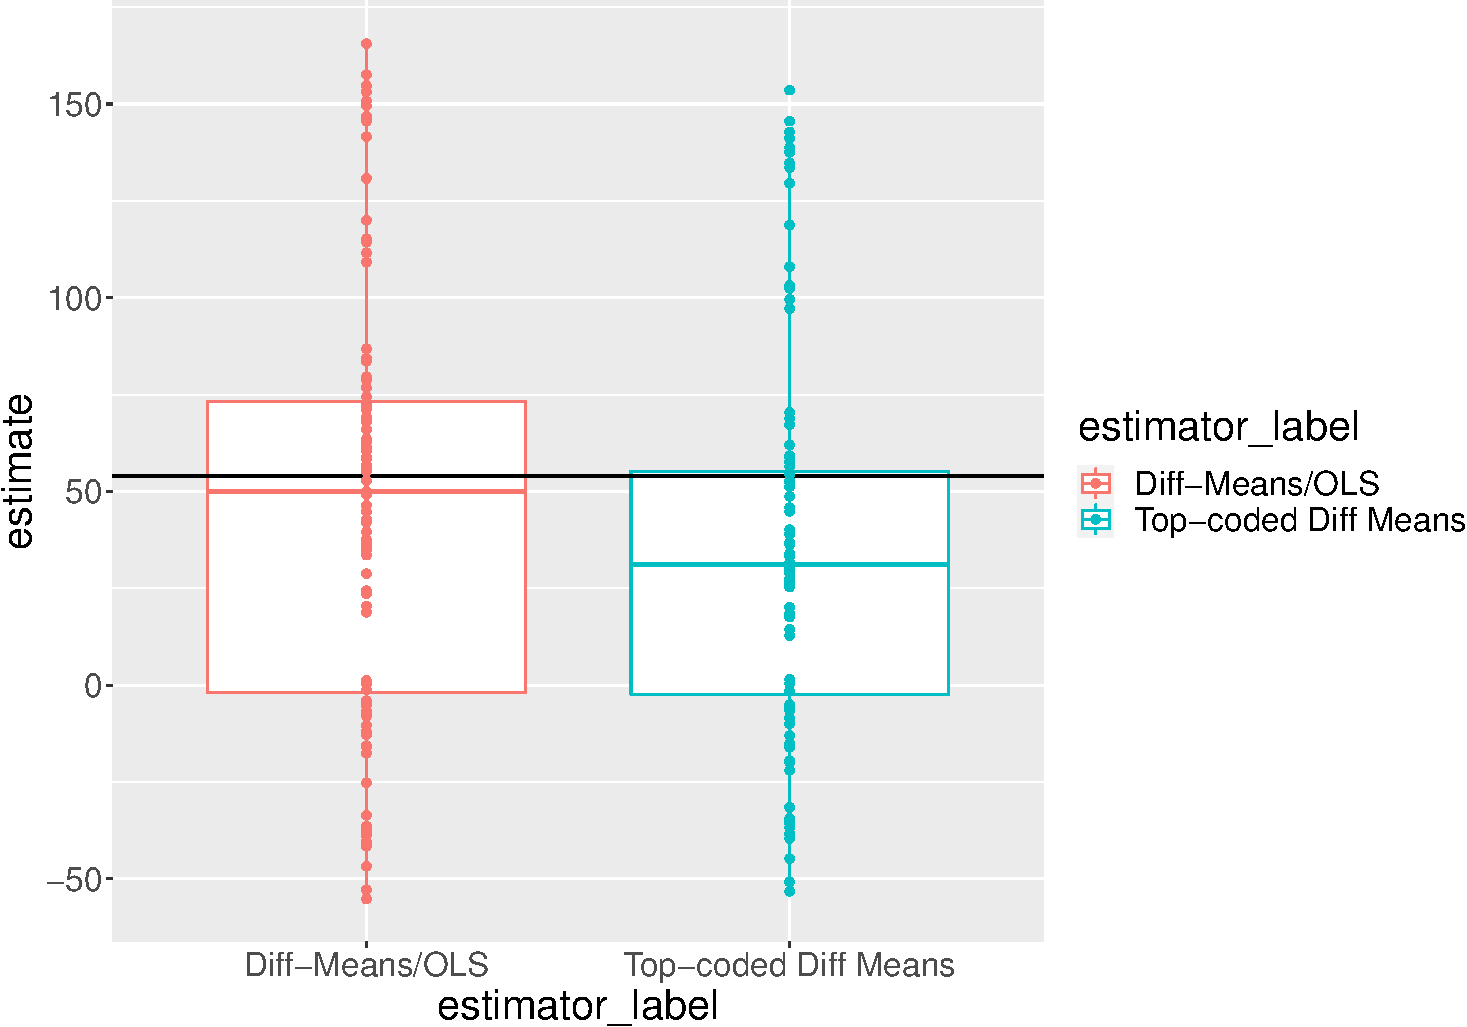
\includegraphics[width=.8\textwidth,]{figs/figsim_plot-1} \normalsize
\end{frame}

\begin{frame}{Which estimator is closer to the truth?}
\protect\hypertarget{which-estimator-is-closer-to-the-truth}{}
One way to choose among estimators is to choose the one that is
\textbf{close to the truth} whenever we use it --- regardless of the
specific randomization.

An ``unbiased'' estimator is one for which \textbf{average of the
estimates across repeated designs} is the same as the truth (or
\(E_R(\hat{\bar{\tau}})=\bar{\tau}\)). An unbiased estimator has ``no
systematic error'' but doesn't guarantee closeness to the truth.

Another measure of closeness is \textbf{root mean squared error} (RMSE)
which records squared distances between the truth and the individual
estimates.

Which estimator is better? (One is closer to the truth on average (RMSE)
and is more precise. The other has no systematic error --- is unbiased.)

\scriptsize
\begin{tabular}{l|l|l|l|l|l}
\hline
Estimator Label & Bias & RMSE & SD Estimate & Mean Se & Power\\
\hline
Diff-Means/OLS & -7.68 & 54.87 & 54.60 & 57.46 & 0.10\\
\hline
Top-coded Diff Means & -18.77 & 53.06 & 49.88 & 51.49 & 0.12\\
\hline
\end{tabular}

\normalsize
\end{frame}

\begin{frame}{Unbiased and biased estimators}
\protect\hypertarget{unbiased-and-biased-estimators}{}
Summary:

\begin{itemize}
\item
  We have a \emph{choice} of both estimands and estimators
\item
  A good estimator performs well regardless of the particular
  randomization of a given design. And \emph{performs well} can mean
  ``unbiased'' and/or ``low mse'' (or ``consistent'' --- which means
  increasingly close to the truth as the sample size increases).
\item
  We can learn about how a given estimator performs in a given study
  using simulation.
\end{itemize}
\end{frame}

\hypertarget{block-randomization}{%
\section{Block randomization}\label{block-randomization}}

\begin{frame}{Block-randomized experiments are a collection of
mini-experiments}
\protect\hypertarget{block-randomized-experiments-are-a-collection-of-mini-experiments}{}
What is the ** ATE** estimand in a block-randomized experiment?

If we think of the unit-level ATE as:
\((1/N) \sum_{i=1}^N y_{i,1} - y_{i,0}\) then we could re-express this
equivalently using the ATE in block \(j\) is \(ATE_j\) as follows:

\[
ATE = \frac{1}{J}\sum^J_{j=1} \sum^{N_j}_{i=1} \frac{y_{i,1} - y_{i,0}}{N_j}  = \sum^J_{j=1} \frac{N_j}{N} ATE_j
\]

And it would be natural to \emph{estimate} this quantity by plugging in
what we can calculate:
\(\widehat{ATE} = \displaystyle\sum^J_{j=1} \frac{N_j}{N} \widehat{ATE}_j\)
\end{frame}

\begin{frame}{Block-randomized experiments are a collection of
mini-experiments}
\protect\hypertarget{block-randomized-experiments-are-a-collection-of-mini-experiments-1}{}
And we could \emph{define} the standard error of the estimator by also
just averaging the within-block standard errors (if our blocks are large
enough):

\(SE(\widehat{ATE}) = \sqrt{\sum^J_{j=1} (\frac{N_{j}}{N})^2SE^2(\widehat{ATE}_j)}\)
\end{frame}

\begin{frame}[fragile]{Estimating the ATE in block-randomized
experiments}
\protect\hypertarget{estimating-the-ate-in-block-randomized-experiments}{}
One approach to estimation simply replaces \(ATE_j\) with
\(\widehat{ATE}\) above:

\scriptsize

\begin{Shaded}
\begin{Highlighting}[]
\FunctionTok{with}\NormalTok{(dat, }\FunctionTok{table}\NormalTok{(b, Z))}
\end{Highlighting}
\end{Shaded}

\begin{verbatim}
   Z
b   0 1
  a 4 2
  b 2 2
\end{verbatim}

\normalsize

We have 6 units in block \texttt{a}, 2 of which are assigned to
treatment, and 4 units in block \texttt{b}, 2 of which are assignment to
treatment.
\end{frame}

\begin{frame}[fragile]{Estimating the ATE in block-randomized
experiments}
\protect\hypertarget{estimating-the-ate-in-block-randomized-experiments-1}{}
One approach to estimation simply replaces \(ATE_j\) with
\(\widehat{ATE}\) above:

\scriptsize

\begin{Shaded}
\begin{Highlighting}[]
\NormalTok{datb }\OtherTok{\textless{}{-}}\NormalTok{ dat }\SpecialCharTok{\%\textgreater{}\%}
  \FunctionTok{group\_by}\NormalTok{(b) }\SpecialCharTok{\%\textgreater{}\%}
  \FunctionTok{summarize}\NormalTok{(}
    \AttributeTok{nb =} \FunctionTok{n}\NormalTok{(), }\AttributeTok{pb =} \FunctionTok{mean}\NormalTok{(Z), }\AttributeTok{estateb =} \FunctionTok{mean}\NormalTok{(Y[Z }\SpecialCharTok{==} \DecValTok{1}\NormalTok{]) }\SpecialCharTok{{-}} \FunctionTok{mean}\NormalTok{(Y[Z }\SpecialCharTok{==} \DecValTok{0}\NormalTok{]),}
    \AttributeTok{ateb =} \FunctionTok{mean}\NormalTok{(y1 }\SpecialCharTok{{-}}\NormalTok{ y0), }\AttributeTok{.groups =} \StringTok{"drop"}
\NormalTok{  )}
\NormalTok{datb}
\end{Highlighting}
\end{Shaded}

\begin{verbatim}
# A tibble: 2 x 5
  b        nb    pb estateb  ateb
  <chr> <int> <dbl>   <dbl> <dbl>
1 a         6 0.333    16.8    60
2 b         4 0.5     246.     45
\end{verbatim}

\begin{Shaded}
\begin{Highlighting}[]
\DocumentationTok{\#\# True ate by block:}
\FunctionTok{with}\NormalTok{(dat, }\FunctionTok{mean}\NormalTok{(y1 }\SpecialCharTok{{-}}\NormalTok{ y0))}
\end{Highlighting}
\end{Shaded}

\begin{verbatim}
[1] 54
\end{verbatim}

\begin{Shaded}
\begin{Highlighting}[]
\DocumentationTok{\#\# This is another way to calculate the true ate}
\FunctionTok{with}\NormalTok{(datb, }\FunctionTok{sum}\NormalTok{(ateb }\SpecialCharTok{*}\NormalTok{ (nb }\SpecialCharTok{/} \FunctionTok{sum}\NormalTok{(nb))))}
\end{Highlighting}
\end{Shaded}

\begin{verbatim}
[1] 54
\end{verbatim}

\normalsize
\end{frame}

\begin{frame}[fragile]{Estimating the ATE in block-randomized
experiments}
\protect\hypertarget{estimating-the-ate-in-block-randomized-experiments-2}{}
One approach is to estimate the overall ATE using block-size weights:

\scriptsize

\begin{Shaded}
\begin{Highlighting}[]
\DocumentationTok{\#\# Showing that difference\_in\_means uses the blocksize weight.}
\NormalTok{e1 }\OtherTok{\textless{}{-}} \FunctionTok{difference\_in\_means}\NormalTok{(Y }\SpecialCharTok{\textasciitilde{}}\NormalTok{ Z, }\AttributeTok{blocks =}\NormalTok{ b, }\AttributeTok{data =}\NormalTok{ dat)}
\NormalTok{e2 }\OtherTok{\textless{}{-}} \FunctionTok{with}\NormalTok{(datb, }\FunctionTok{sum}\NormalTok{(estateb }\SpecialCharTok{*}\NormalTok{ (nb }\SpecialCharTok{/} \FunctionTok{sum}\NormalTok{(nb))))}
\FunctionTok{c}\NormalTok{(}\FunctionTok{coef}\NormalTok{(e1)[[}\StringTok{"Z"}\NormalTok{]], e2)}
\end{Highlighting}
\end{Shaded}

\begin{verbatim}
[1] 108.2 108.2
\end{verbatim}

\normalsize
\end{frame}

\begin{frame}[fragile]{Estimating the ATE in block-randomized
experiments}
\protect\hypertarget{estimating-the-ate-in-block-randomized-experiments-3}{}
Notice that this is \textbf{not} the same as either of the following:

\scriptsize

\begin{Shaded}
\begin{Highlighting}[]
\DocumentationTok{\#\# Ignoring blocks}
\NormalTok{e3 }\OtherTok{\textless{}{-}} \FunctionTok{lm}\NormalTok{(Y }\SpecialCharTok{\textasciitilde{}}\NormalTok{ Z, }\AttributeTok{data =}\NormalTok{ dat)}
\FunctionTok{coef}\NormalTok{(e3)[[}\StringTok{"Z"}\NormalTok{]]}
\end{Highlighting}
\end{Shaded}

\begin{verbatim}
[1] 131.8
\end{verbatim}

\begin{Shaded}
\begin{Highlighting}[]
\DocumentationTok{\#\# With block fixed effects}
\NormalTok{e4 }\OtherTok{\textless{}{-}} \FunctionTok{lm}\NormalTok{(Y }\SpecialCharTok{\textasciitilde{}}\NormalTok{ Z }\SpecialCharTok{+}\NormalTok{ block, }\AttributeTok{data =}\NormalTok{ dat)}
\FunctionTok{coef}\NormalTok{(e4)[[}\StringTok{"Z"}\NormalTok{]]}
\end{Highlighting}
\end{Shaded}

\begin{verbatim}
[1] 114.8
\end{verbatim}

\normalsize

How do they differ? (The first ignores the blocks. The second uses a
different set of weights that are created by use of ``fixed effects'' or
``indicator'' or ``dummy'' variables.)
\end{frame}

\begin{frame}[fragile]{Which estimator should we use?}
\protect\hypertarget{which-estimator-should-we-use}{}
We now have three estimators each with a different estimate (imagining
they all target the same estimand):

\scriptsize

\begin{Shaded}
\begin{Highlighting}[]
\FunctionTok{c}\NormalTok{(}\FunctionTok{coef}\NormalTok{(e1)[[}\StringTok{"Z"}\NormalTok{]], }\FunctionTok{coef}\NormalTok{(e3)[[}\StringTok{"Z"}\NormalTok{]], }\FunctionTok{coef}\NormalTok{(e4)[[}\StringTok{"Z"}\NormalTok{]])}
\end{Highlighting}
\end{Shaded}

\begin{verbatim}
[1] 108.2 131.8 114.8
\end{verbatim}

\normalsize

Which estimator should we use for this design? We can set up a
DeclareDesign simulation to figure this out.

\scriptsize

\begin{Shaded}
\begin{Highlighting}[]
\DocumentationTok{\#\# declare a new base design that includes the block indicator b}
\NormalTok{base\_design\_blocks }\OtherTok{\textless{}{-}}
  \CommentTok{\# declare the population}
  \FunctionTok{declare\_population}\NormalTok{(dat[, }\FunctionTok{c}\NormalTok{(}\StringTok{"b"}\NormalTok{, }\StringTok{"y0"}\NormalTok{, }\StringTok{"y1"}\NormalTok{)]) }\SpecialCharTok{+}
  \CommentTok{\# tell DD that b indicates block and to assign 2 treated units in each block}
  \FunctionTok{declare\_assignment}\NormalTok{(}\AttributeTok{m =} \DecValTok{2}\NormalTok{, }\AttributeTok{blocks =}\NormalTok{ b) }\SpecialCharTok{+}
  \CommentTok{\# relationship of potential outcomes to observed outcome}
  \FunctionTok{declare\_potential\_outcomes}\NormalTok{(Y }\SpecialCharTok{\textasciitilde{}}\NormalTok{ Z }\SpecialCharTok{*}\NormalTok{ y1 }\SpecialCharTok{+}\NormalTok{ (}\DecValTok{1} \SpecialCharTok{{-}}\NormalTok{ Z) }\SpecialCharTok{*}\NormalTok{ y0) }\SpecialCharTok{+}
  \CommentTok{\# observed outcome and treatment assignment}
  \FunctionTok{declare\_reveal}\NormalTok{(Y, Z)}
\end{Highlighting}
\end{Shaded}

\normalsize
\end{frame}

\begin{frame}[fragile]{Which estimator should we use?}
\protect\hypertarget{which-estimator-should-we-use-1}{}
\scriptsize

\begin{Shaded}
\begin{Highlighting}[]
\CommentTok{\# the estimand is the average treatment effect}
\NormalTok{estimandATEb }\OtherTok{\textless{}{-}} \FunctionTok{declare\_estimand}\NormalTok{(}\AttributeTok{ATE =} \FunctionTok{mean}\NormalTok{(Y\_Z\_1 }\SpecialCharTok{{-}}\NormalTok{ Y\_Z\_0))}

\CommentTok{\# three different estimators}
\NormalTok{est1 }\OtherTok{\textless{}{-}} \FunctionTok{declare\_estimator}\NormalTok{(Y }\SpecialCharTok{\textasciitilde{}}\NormalTok{ Z,}
  \AttributeTok{estimand =}\NormalTok{ estimandATEb, }\AttributeTok{model =}\NormalTok{ lm\_robust,}
  \AttributeTok{label =} \StringTok{"Ignores Blocks"}
\NormalTok{)}
\NormalTok{est2 }\OtherTok{\textless{}{-}} \FunctionTok{declare\_estimator}\NormalTok{(Y }\SpecialCharTok{\textasciitilde{}}\NormalTok{ Z,}
  \AttributeTok{estimand =}\NormalTok{ estimandATEb, }\AttributeTok{model =}\NormalTok{ difference\_in\_means, }\AttributeTok{blocks =}\NormalTok{ b,}
  \AttributeTok{label =} \StringTok{"DiM: Block{-}Size Weights"}
\NormalTok{)}
\NormalTok{est3 }\OtherTok{\textless{}{-}} \FunctionTok{declare\_estimator}\NormalTok{(Y }\SpecialCharTok{\textasciitilde{}}\NormalTok{ Z,}
  \AttributeTok{estimand =}\NormalTok{ estimandATEb, }\AttributeTok{model =}\NormalTok{ lm\_robust,}
  \AttributeTok{weights =}\NormalTok{ (Z }\SpecialCharTok{/}\NormalTok{ Z\_cond\_prob) }\SpecialCharTok{+}\NormalTok{ ((}\DecValTok{1} \SpecialCharTok{{-}}\NormalTok{ Z) }\SpecialCharTok{/}\NormalTok{ (Z\_cond\_prob)),}
  \AttributeTok{label =} \StringTok{"LM: Block Size Weights"}
\NormalTok{)}
\end{Highlighting}
\end{Shaded}

\normalsize
\end{frame}

\begin{frame}[fragile]{Which estimator should we use?}
\protect\hypertarget{which-estimator-should-we-use-2}{}
\scriptsize

\begin{Shaded}
\begin{Highlighting}[]
\CommentTok{\# two more estimators}
\NormalTok{est4 }\OtherTok{\textless{}{-}} \FunctionTok{declare\_estimator}\NormalTok{(Y }\SpecialCharTok{\textasciitilde{}}\NormalTok{ Z,}
  \AttributeTok{estimand =}\NormalTok{ estimandATEb,}
  \AttributeTok{model =}\NormalTok{ lm\_robust, }\AttributeTok{fixed\_effects =} \SpecialCharTok{\textasciitilde{}}\NormalTok{b, }\AttributeTok{label =} \StringTok{"Precision Weights"}
\NormalTok{)}
\NormalTok{est5 }\OtherTok{\textless{}{-}} \FunctionTok{declare\_estimator}\NormalTok{(Y }\SpecialCharTok{\textasciitilde{}}\NormalTok{ Z }\SpecialCharTok{+}\NormalTok{ b,}
  \AttributeTok{estimand =}\NormalTok{ estimandATEb,}
  \AttributeTok{model =}\NormalTok{ lm\_robust, }\AttributeTok{label =} \StringTok{"Precision Weights (LSDV)"}
\NormalTok{)}

\DocumentationTok{\#\# new design object has the base design, the estimand, and five estimators}
\NormalTok{design\_blocks }\OtherTok{\textless{}{-}}\NormalTok{ base\_design\_blocks }\SpecialCharTok{+}\NormalTok{ estimandATEb }\SpecialCharTok{+}
\NormalTok{  est1 }\SpecialCharTok{+}\NormalTok{ est2 }\SpecialCharTok{+}\NormalTok{ est3 }\SpecialCharTok{+}\NormalTok{ est4 }\SpecialCharTok{+}\NormalTok{ est5}
\end{Highlighting}
\end{Shaded}

\normalsize

Then we will run 10,000 simulations (reassign treatment 10,000 times)
and summarize the estimates produced by each of these five estimators.
\end{frame}

\begin{frame}{Which estimator should we use?}
\protect\hypertarget{which-estimator-should-we-use-3}{}
\scriptsize\normalsize

\scriptsize\normalsize

How should we interpret this plot?

\scriptsize

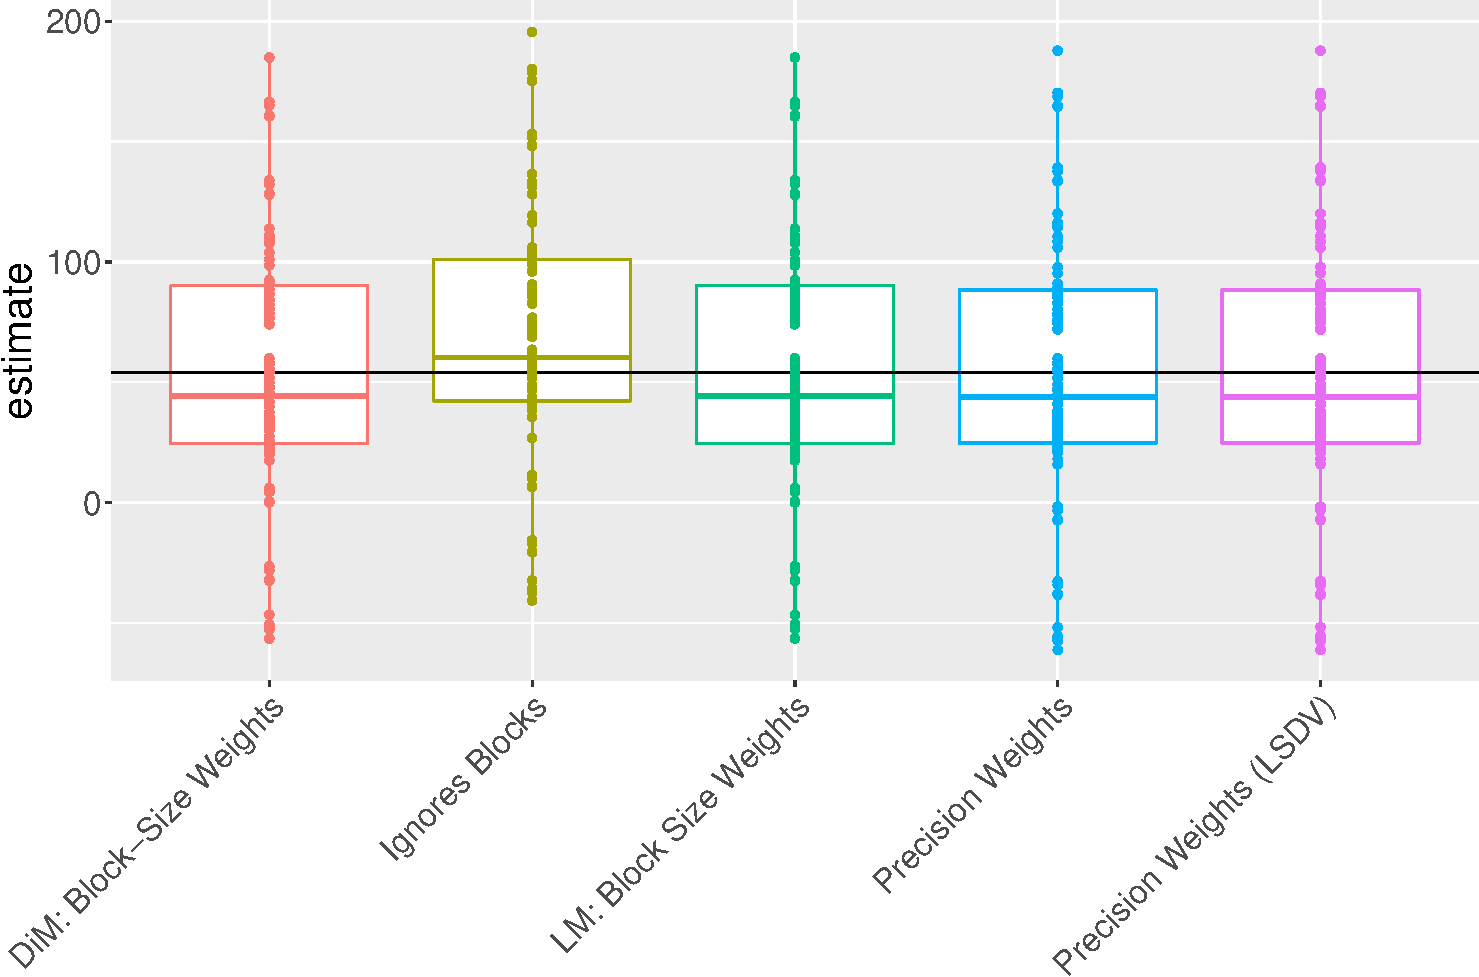
\includegraphics[width=.9\textwidth,]{figs/figsim_plot2-1} \normalsize
\end{frame}

\begin{frame}{Which estimator is closer to the truth?}
\protect\hypertarget{which-estimator-is-closer-to-the-truth-1}{}
Which estimator works better on this design and these data?

\scriptsize
\begin{tabular}{l|l|l|l|l|l|l}
\hline
Estimator & Bias & RMSE & SD Est & Mean SE & Power & Coverage\\
\hline
DiM: Block-Size Weights & -0.63 & 53.08 & 53.11 & 51.90 & 0.22 & 0.77\\
\hline
Ignores Blocks & 14.48 & 55.23 & 53.33 & 60.79 & 0.10 & 0.97\\
\hline
LM: Block Size Weights & -0.63 & 53.08 & 53.11 & 60.57 & 0.08 & 0.93\\
\hline
Precision Weights & -1.02 & 55.39 & 55.40 & 56.96 & 0.11 & 0.92\\
\hline
Precision Weights (LSDV) & -1.02 & 55.39 & 55.40 & 56.96 & 0.11 & 0.92\\
\hline
\end{tabular}

\normalsize

Notice that the coverage is not always at 95\% in all cases. We used
10,000 simulations so simulation error is around
\(\pm 2 \sqrt{p(1-p)/10000}\) or, say, for coverage calculated as .93, a
different simulation could have easily produced 0.9249 or 0.9351 (or
would rarely have produced coverage numbers outside that range just by
chance).
\end{frame}

\hypertarget{cluster-randomization}{%
\section{Cluster randomization}\label{cluster-randomization}}

\begin{frame}[allowframebreaks]{In cluster-randomized experiments, units
are randomized as a group (cluster) to treatment}
\protect\hypertarget{in-cluster-randomized-experiments-units-are-randomized-as-a-group-cluster-to-treatment}{}
\begin{itemize}
\tightlist
\item
  \textbf{Example 1:} an intervention is randomized across
  neighborhoods, so \textbf{all} households in a neighborhood will be
  assigned to the same treatment condition, but different neighborhoods
  will be assigned different treatment conditions.
\item
  \textbf{Example 2:} an intervention is randomized across people and
  each person is measured four times after treatment, so our data
  contain four rows per person.
\item
  \textbf{Not An Example 1:} Neighborhoods are chosen for the study.
  Within each neighborhood about half of the people are assigned to
  treatment and half to control. (What kind of study is this? It is not
  a cluster-randomized study.)
\item
  \textbf{Not an Example 2:} an intervention is randomized to some
  neighborhoods and not to others, the outcomes include measurements of
  neighborhood-level trust in government and total land area in the
  neighborhood devoted to gardens. (Sometimes a cluster randomized
  experiment can be turned into a simple randomized experiment. Or may
  contain more than one possible approach to analysis and
  interpretation.)
\end{itemize}

How might the distribution of test statistics and estimators differ from
an experiment where individual units (not clusters) are randomized?
\end{frame}

\begin{frame}{Estimating the ATE in cluster-randomized experiments}
\protect\hypertarget{estimating-the-ate-in-cluster-randomized-experiments}{}
Bias problems in cluster-randomized experiments:

\begin{itemize}
\item
  When clusters are the same size, the usual difference-in-means
  estimator is unbiased.
\item
  But be careful when clusters have different numbers of units or you
  have very few clusters because then treatment effects may be
  correlated with cluster size.
\item
  When cluster size is related to potential outcomes, the usual
  difference-in-means estimator is biased.
  \url{https://declaredesign.org/blog/bias-cluster-randomized-trials.html}
\end{itemize}
\end{frame}

\begin{frame}[fragile,allowframebreaks]{Estimating the SE for the ATE in
cluster-randomized experiments}
\protect\hypertarget{estimating-the-se-for-the-ate-in-cluster-randomized-experiments}{}
\begin{itemize}
\item
  \textbf{Misleading statistical inferences:} The default SE will
  generally underestimate precision in such designs and thus produce
  tests with false positive rates that are too high (or equivalently
  confidence intervals coverage rates that are too low).
\item
  The ``cluster robust standard errors'' implemented in common software
  work well \textbf{when the number of clusters is large} (like more
  than 50 in some simulation studies).
\item
  The default cluster-appropriate standard errors in \texttt{lm\_robust}
  (the \texttt{CR2} SEs) work better than the common approach in Stata
  (as of this writing).
\item
  The wild bootstrap helps control error rates but gives up statistical
  power much more than perhaps necessary in a cluster randomized study
  where direct randomization inference is possible.
\item
  When in doubt, one can produce \(p\)-values by direct simulation
  (direct randomization inference) to see if they agree with one of the
  cluster robust approaches.
\end{itemize}

Overall, it is worth simulating to study the performance of your
estimators, tests, and confidence intervals if you have any worries or
doubts.
\end{frame}

\begin{frame}[fragile]{An example of estimation}
\protect\hypertarget{an-example-of-estimation}{}
\scriptsize\normalsize

Imagine we had data from 10 clusters with either 100 people (for 2
clusters) or 10 people per cluster (for 8 clusters). The total size of
the data is 280.

\scriptsize

\begin{verbatim}
# A tibble: 6 x 6
# Groups:   clus_id [2]
  clus_id indiv Y_Z_0 Y_Z_1     Z     Y
  <chr>   <chr> <dbl> <dbl> <int> <dbl>
1 01      010    4.51  4.61     0  4.51
2 01      035    4.63  4.73     0  4.63
3 01      068    4.76  4.86     0  4.76
4 03      205    3.13  4.13     1  4.13
5 03      206    2.41  3.41     1  3.41
6 03      208    2.95  3.95     1  3.95
\end{verbatim}

\normalsize
\end{frame}

\begin{frame}[fragile]{An example of estimation}
\protect\hypertarget{an-example-of-estimation-1}{}
Which estimator should we use? Which test should we use? On what basis
should we choose among these approaches?

\scriptsize

\begin{Shaded}
\begin{Highlighting}[]
\NormalTok{lmc1 }\OtherTok{\textless{}{-}} \FunctionTok{lm\_robust}\NormalTok{(Y }\SpecialCharTok{\textasciitilde{}}\NormalTok{ Z, }\AttributeTok{data =}\NormalTok{ dat1)}
\NormalTok{lmc2 }\OtherTok{\textless{}{-}} \FunctionTok{lm\_robust}\NormalTok{(Y }\SpecialCharTok{\textasciitilde{}}\NormalTok{ Z, }\AttributeTok{clusters =}\NormalTok{ clus\_id, }\AttributeTok{data =}\NormalTok{ dat1)}
\NormalTok{lmc3 }\OtherTok{\textless{}{-}} \FunctionTok{lm\_robust}\NormalTok{(Y }\SpecialCharTok{\textasciitilde{}}\NormalTok{ Z }\SpecialCharTok{+}\NormalTok{ cl\_sizeF, }\AttributeTok{clusters =}\NormalTok{ clus\_id, }\AttributeTok{data =}\NormalTok{ dat1)}
\FunctionTok{tidy}\NormalTok{(lmc1)[}\DecValTok{2}\NormalTok{, ]}
\end{Highlighting}
\end{Shaded}

\begin{verbatim}
  term estimate std.error statistic p.value conf.low conf.high  df outcome
2    Z   0.3024    0.1207     2.504 0.01284  0.06471    0.5401 278       Y
\end{verbatim}

\begin{Shaded}
\begin{Highlighting}[]
\FunctionTok{tidy}\NormalTok{(lmc2)[}\DecValTok{2}\NormalTok{, ]}
\end{Highlighting}
\end{Shaded}

\begin{verbatim}
  term estimate std.error statistic p.value conf.low conf.high    df outcome
2    Z   0.3024     1.079    0.2804   0.796   -2.969     3.574 3.282       Y
\end{verbatim}

\begin{Shaded}
\begin{Highlighting}[]
\FunctionTok{tidy}\NormalTok{(lmc3)[}\DecValTok{2}\NormalTok{, ]}
\end{Highlighting}
\end{Shaded}

\begin{verbatim}
  term estimate std.error statistic p.value conf.low conf.high    df outcome
2    Z   0.3024     0.306    0.9882  0.4386   -1.194     1.799 1.769       Y
\end{verbatim}

\normalsize
\end{frame}

\begin{frame}[fragile]{Use simulation to assess estimators and tests}
\protect\hypertarget{use-simulation-to-assess-estimators-and-tests}{}
If you look at the code for the slides you will see that we simulate the
design 5000 times, each time calculating an estimate and confidence
interval for different estimators of the ATE.

What should we learn from this table? (Coverage? \texttt{sd\_estimate}
versus \texttt{mean\_se}).

\scriptsize\normalsize

\scriptsize\normalsize

\scriptsize\normalsize

\scriptsize

\begin{table}

\caption{\label{tab:showresclus1}Estimator and Test Performance in 5000 simulations of the cluster randomized design for different estimators and confidence intervals}
\centering
\begin{tabular}[t]{lrrr}
\toprule
estimator\_label & coverage & sd\_estimate & mean\_se\\
\midrule
Y\textasciitilde{}Z, CR2 & 0.56 & 1.07 & 0.72\\
Y\textasciitilde{}Z, cl\_size fe, CR2 & 0.75 & 0.35 & 0.30\\
Y\textasciitilde{}Z, HC2 & 0.56 & 1.07 & 0.13\\
Y\textasciitilde{}Z, IID & 0.56 & 1.07 & 0.12\\
Y\textasciitilde{}Z, weight=clus\_size, CR2 & 0.56 & 1.22 & 0.84\\
Y\textasciitilde{}Z*I(cl\_size-mean(cl\_size)), CR2 & 0.75 & 1.61 & 0.06\\
Y\textasciitilde{}Z+cl\_sizeF, CR2 & 0.75 & 0.35 & 0.30\\
\bottomrule
\end{tabular}
\end{table}

\normalsize
\end{frame}

\begin{frame}{Use simulation to assess estimators and tests}
\protect\hypertarget{use-simulation-to-assess-estimators-and-tests-1}{}
What should we learn from this table? (Bias? Closeness to truth?)

\scriptsize

\begin{table}

\caption{\label{tab:showresclus2}Estimator and Test Performance in 5000 simulations of the cluster randomized design for different estimators and confidence intervals}
\centering
\begin{tabular}[t]{lrr}
\toprule
estimator\_label & bias & rmse\\
\midrule
Y\textasciitilde{}Z, CR2 & 0.132 & 1.079\\
Y\textasciitilde{}Z, cl\_size fe, CR2 & 0.278 & 0.448\\
Y\textasciitilde{}Z, HC2 & 0.132 & 1.079\\
Y\textasciitilde{}Z, IID & 0.132 & 1.079\\
Y\textasciitilde{}Z, weight=clus\_size, CR2 & -0.014 & 1.224\\
Y\textasciitilde{}Z*I(cl\_size-mean(cl\_size)), CR2 & 0.836 & 1.814\\
Y\textasciitilde{}Z+cl\_sizeF, CR2 & 0.278 & 0.448\\
\bottomrule
\end{tabular}
\end{table}

\normalsize
\end{frame}

\begin{frame}{Use simulation to assess estimators and tests}
\protect\hypertarget{use-simulation-to-assess-estimators-and-tests-2}{}
How should we interpret this plot?

\scriptsize

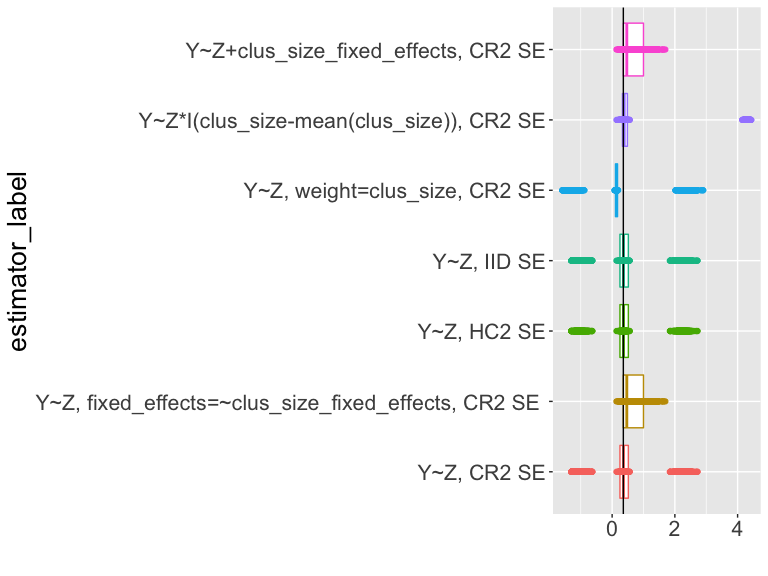
\includegraphics[width=.95\textwidth,]{figs/figsim_plot_clus-1}
\normalsize
\end{frame}

\begin{frame}{Summary of estimation and testing in cluster-randomized
trials}
\protect\hypertarget{summary-of-estimation-and-testing-in-cluster-randomized-trials}{}
\begin{itemize}
\item
  Cluster randomized trials pose special problems for standard
  approaches to estimation and testing.
\item
  If randomization is at the cluster level, then uncertainty arises from
  the cluster level randomization.
\item
  If we have enough clusters, then one of the ``cluster robust''
  standard errors can help us produce confidence intervals with correct
  coverage. \textbf{Cluster robust standard errors require many
  clusters}.
\item
  If cluster size (or characteristic) is related to effect size, then we
  can have bias (and we need to adjust somehow).
\end{itemize}
\end{frame}

\hypertarget{binary-outcomes}{%
\section{Binary outcomes}\label{binary-outcomes}}

\begin{frame}[fragile]{Binary outcomes: Set up our data for simulation
in DeclareDesign}
\protect\hypertarget{binary-outcomes-set-up-our-data-for-simulation-in-declaredesign}{}
\scriptsize

\begin{Shaded}
\begin{Highlighting}[]
\CommentTok{\# population size}
\NormalTok{N }\OtherTok{\textless{}{-}} \DecValTok{20}
\CommentTok{\# declare the population}
\NormalTok{thepop\_bin }\OtherTok{\textless{}{-}} \FunctionTok{declare\_population}\NormalTok{(}
  \AttributeTok{N =}\NormalTok{ N, }\AttributeTok{x1 =} \FunctionTok{draw\_binary}\NormalTok{(}\AttributeTok{prob =}\NormalTok{ .}\DecValTok{5}\NormalTok{, }\AttributeTok{N =}\NormalTok{ N),}
  \AttributeTok{x2 =} \FunctionTok{rnorm}\NormalTok{(N)}
\NormalTok{)}
\CommentTok{\# declare the potential outcomes}
\NormalTok{thepo\_bin }\OtherTok{\textless{}{-}} \FunctionTok{declare\_potential\_outcomes}\NormalTok{(Y }\SpecialCharTok{\textasciitilde{}} \FunctionTok{rbinom}\NormalTok{(}
  \AttributeTok{n =}\NormalTok{ N, }\AttributeTok{size =} \DecValTok{1}\NormalTok{,}
  \AttributeTok{prob =} \FloatTok{0.5} \SpecialCharTok{+} \FloatTok{0.05} \SpecialCharTok{*}\NormalTok{ Z }\SpecialCharTok{+}\NormalTok{ x1 }\SpecialCharTok{*}\NormalTok{ .}\DecValTok{05}
\NormalTok{))}
\CommentTok{\# two possible targets: difference in means or difference in log{-}odds}
\NormalTok{thetarget\_ate }\OtherTok{\textless{}{-}} \FunctionTok{declare\_estimand}\NormalTok{(}\AttributeTok{ate =} \FunctionTok{mean}\NormalTok{(Y\_Z\_1 }\SpecialCharTok{{-}}\NormalTok{ Y\_Z\_0))}
\NormalTok{thetarget\_logodds }\OtherTok{\textless{}{-}} \FunctionTok{declare\_estimand}\NormalTok{(}
  \AttributeTok{logodds =} \FunctionTok{log}\NormalTok{(}\FunctionTok{mean}\NormalTok{(Y\_Z\_1) }\SpecialCharTok{/}\NormalTok{ (}\DecValTok{1} \SpecialCharTok{{-}} \FunctionTok{mean}\NormalTok{(Y\_Z\_1))) }\SpecialCharTok{{-}}
    \FunctionTok{log}\NormalTok{(}\FunctionTok{mean}\NormalTok{(Y\_Z\_0) }\SpecialCharTok{/}\NormalTok{ (}\DecValTok{1} \SpecialCharTok{{-}} \FunctionTok{mean}\NormalTok{(Y\_Z\_0)))}
\NormalTok{)}
\end{Highlighting}
\end{Shaded}

\normalsize
\end{frame}

\begin{frame}[fragile]{Binary outcomes: Set up our data for simulation
in DeclareDesign}
\protect\hypertarget{binary-outcomes-set-up-our-data-for-simulation-in-declaredesign-1}{}
\scriptsize

\begin{Shaded}
\begin{Highlighting}[]
\CommentTok{\# declare how treatment is assigned}
\CommentTok{\# m units are assigned to levels of treatment Z}
\NormalTok{theassign\_bin }\OtherTok{\textless{}{-}} \FunctionTok{declare\_assignment}\NormalTok{(}\AttributeTok{m =} \FunctionTok{floor}\NormalTok{(N }\SpecialCharTok{/} \DecValTok{3}\NormalTok{))}
\CommentTok{\# declare what outcome values are revealed for possible values of Z}
\NormalTok{thereveal\_bin }\OtherTok{\textless{}{-}} \FunctionTok{declare\_reveal}\NormalTok{(Y, Z)}
\CommentTok{\# pull this all together: population, potential outcomes, assignment,}
\DocumentationTok{\#\# outcome values connected to Z}
\NormalTok{des\_bin }\OtherTok{\textless{}{-}}\NormalTok{ thepop\_bin }\SpecialCharTok{+}\NormalTok{ thepo\_bin }\SpecialCharTok{+}\NormalTok{ theassign\_bin }\SpecialCharTok{+}\NormalTok{ thereveal\_bin}
\CommentTok{\# then make one draw (randomize treatment once)}
\FunctionTok{set.seed}\NormalTok{(}\DecValTok{12345}\NormalTok{)}
\NormalTok{dat2 }\OtherTok{\textless{}{-}} \FunctionTok{draw\_data}\NormalTok{(des\_bin)}
\end{Highlighting}
\end{Shaded}

\normalsize
\end{frame}

\begin{frame}[fragile]{Binary outcomes: Estimands I}
\protect\hypertarget{binary-outcomes-estimands-i}{}
How would we interpret the following true quantities or estimands?
(\texttt{Y\_Z\_1}, \texttt{Y\_Z\_0} are potential outcomes, \texttt{Y}
is observed, \texttt{x1}, \texttt{x2} are covariates, \texttt{Z} is
treatment assignment. Here \(N\)=20.

\scriptsize

\begin{Shaded}
\begin{Highlighting}[]
\DocumentationTok{\#\# Look at the first 6 observations only:}
\FunctionTok{head}\NormalTok{(dat2[, }\SpecialCharTok{{-}}\DecValTok{7}\NormalTok{])}
\end{Highlighting}
\end{Shaded}

\begin{verbatim}
  ID x1      x2 Y_Z_0 Y_Z_1 Z Y
1 01  1 -0.1162     0     1 0 0
2 02  1  1.8173     0     1 1 1
3 03  1  0.3706     0     1 0 0
4 04  1  0.5202     1     1 0 1
5 05  0 -0.7505     1     0 1 0
6 06  0  0.8169     0     1 0 0
\end{verbatim}

\normalsize
\end{frame}

\begin{frame}[fragile]{Binary outcomes: Estimands II}
\protect\hypertarget{binary-outcomes-estimands-ii}{}
How would we interpret the following true quantities or estimands?
(\texttt{Y\_Z\_1}, \texttt{Y\_Z\_0} are potential outcomes, \texttt{Y}
is observed, \texttt{x1}, \texttt{x2} are covariates, \texttt{Z} is
treatment assignment. Here \(N\)=20.

\scriptsize

\begin{Shaded}
\begin{Highlighting}[]
\NormalTok{ate\_bin }\OtherTok{\textless{}{-}} \FunctionTok{with}\NormalTok{(dat2, }\FunctionTok{mean}\NormalTok{(Y\_Z\_1 }\SpecialCharTok{{-}}\NormalTok{ Y\_Z\_0))}
\NormalTok{bary1 }\OtherTok{\textless{}{-}} \FunctionTok{mean}\NormalTok{(dat2}\SpecialCharTok{$}\NormalTok{Y\_Z\_1)}
\NormalTok{bary0 }\OtherTok{\textless{}{-}} \FunctionTok{mean}\NormalTok{(dat2}\SpecialCharTok{$}\NormalTok{Y\_Z\_0)}
\NormalTok{diff\_log\_odds\_bin }\OtherTok{\textless{}{-}} \FunctionTok{with}\NormalTok{(}
\NormalTok{  dat2,}
  \FunctionTok{log}\NormalTok{(bary1 }\SpecialCharTok{/}\NormalTok{ (}\DecValTok{1} \SpecialCharTok{{-}}\NormalTok{ bary1)) }\SpecialCharTok{{-}} \FunctionTok{log}\NormalTok{(bary0 }\SpecialCharTok{/}\NormalTok{ (}\DecValTok{1} \SpecialCharTok{{-}}\NormalTok{ bary0))}
\NormalTok{)}
\FunctionTok{c}\NormalTok{(}
  \AttributeTok{bary1 =}\NormalTok{ bary1, }\AttributeTok{bary0 =}\NormalTok{ bary0, }\AttributeTok{true\_ate =}\NormalTok{ ate\_bin,}
  \AttributeTok{true\_diff\_log\_odds =}\NormalTok{ diff\_log\_odds\_bin}
\NormalTok{)}
\end{Highlighting}
\end{Shaded}

\begin{verbatim}
             bary1              bary0           true_ate true_diff_log_odds 
              0.55               0.55               0.00               0.00 
\end{verbatim}

\normalsize
\end{frame}

\begin{frame}{Binary outcomes: Estimands III}
\protect\hypertarget{binary-outcomes-estimands-iii}{}
Do you want to estimate the difference in log-odds?

\begin{equation}
\delta = \log \frac{\bar{y}_{1}}{1-\bar{y}_{1}} - \log \frac{ \bar{y}_0}{1- \bar{y}_0}
\end{equation}

Or the difference in proportions?

\begin{equation}
\bar{\tau} = \bar{y}_{1} - \bar{y}_0
\end{equation}

Recall that \(\bar{y}_1\) is the \emph{proportion} of \(y_{1}=1\) in the
data.

\protect\hyperlink{ref-freedman2008randomization}{Freedman}
(\protect\hyperlink{ref-freedman2008randomization}{2008b}) shows us that
the logit coefficient estimator is a biased estimator of the difference
in log-odds estimand. He also shows an unbiased estimator of that
estimand.

We know that the difference of proportions in the sample should be an
unbiased estimator of the difference of proportions.
\end{frame}

\begin{frame}[fragile]{An example of estimation I}
\protect\hypertarget{an-example-of-estimation-i}{}
How should we interpret the following estimates? (What does the
difference of means estimator require in terms of assumptions? What does
the logistic regression estimator require in terms of assumptions?)

\scriptsize

\begin{Shaded}
\begin{Highlighting}[]
\NormalTok{lmbin1 }\OtherTok{\textless{}{-}} \FunctionTok{lm\_robust}\NormalTok{(Y }\SpecialCharTok{\textasciitilde{}}\NormalTok{ Z, }\AttributeTok{data =}\NormalTok{ dat2)}
\NormalTok{glmbin1 }\OtherTok{\textless{}{-}} \FunctionTok{glm}\NormalTok{(Y }\SpecialCharTok{\textasciitilde{}}\NormalTok{ Z, }\AttributeTok{data =}\NormalTok{ dat2, }\AttributeTok{family =} \FunctionTok{binomial}\NormalTok{(}\AttributeTok{link =} \StringTok{"logit"}\NormalTok{))}

\FunctionTok{tidy}\NormalTok{(lmbin1)[}\DecValTok{2}\NormalTok{, ]}
\end{Highlighting}
\end{Shaded}

\begin{verbatim}
  term estimate std.error statistic p.value conf.low conf.high df outcome
2    Z  -0.4048    0.2159    -1.875 0.07716  -0.8584   0.04884 18       Y
\end{verbatim}

\begin{Shaded}
\begin{Highlighting}[]
\FunctionTok{tidy}\NormalTok{(glmbin1)[}\DecValTok{2}\NormalTok{, ]}
\end{Highlighting}
\end{Shaded}

\begin{verbatim}
# A tibble: 1 x 5
  term  estimate std.error statistic p.value
  <chr>    <dbl>     <dbl>     <dbl>   <dbl>
1 Z        -1.90      1.22     -1.55   0.120
\end{verbatim}

\normalsize
\end{frame}

\begin{frame}[fragile]{An example of estimation II}
\protect\hypertarget{an-example-of-estimation-ii}{}
What about with covariates? Why use covariates?

\scriptsize

\begin{Shaded}
\begin{Highlighting}[]
\NormalTok{lmbin2 }\OtherTok{\textless{}{-}} \FunctionTok{lm\_robust}\NormalTok{(Y }\SpecialCharTok{\textasciitilde{}}\NormalTok{ Z }\SpecialCharTok{+}\NormalTok{ x1, }\AttributeTok{data =}\NormalTok{ dat2)}
\NormalTok{glmbin2 }\OtherTok{\textless{}{-}} \FunctionTok{glm}\NormalTok{(Y }\SpecialCharTok{\textasciitilde{}}\NormalTok{ Z }\SpecialCharTok{+}\NormalTok{ x1, }\AttributeTok{data =}\NormalTok{ dat2, }\AttributeTok{family =} \FunctionTok{binomial}\NormalTok{(}\AttributeTok{link =} \StringTok{"logit"}\NormalTok{))}

\FunctionTok{tidy}\NormalTok{(lmbin2)[}\DecValTok{2}\NormalTok{, ]}
\end{Highlighting}
\end{Shaded}

\begin{verbatim}
  term estimate std.error statistic p.value conf.low conf.high df outcome
2    Z  -0.4058    0.2179    -1.862 0.07996  -0.8656   0.05398 17       Y
\end{verbatim}

\begin{Shaded}
\begin{Highlighting}[]
\FunctionTok{tidy}\NormalTok{(glmbin2)[}\DecValTok{2}\NormalTok{, ]}
\end{Highlighting}
\end{Shaded}

\begin{verbatim}
# A tibble: 1 x 5
  term  estimate std.error statistic p.value
  <chr>    <dbl>     <dbl>     <dbl>   <dbl>
1 Z        -1.90      1.22     -1.55   0.120
\end{verbatim}

\normalsize
\end{frame}

\begin{frame}[fragile]{An example of estimation III}
\protect\hypertarget{an-example-of-estimation-iii}{}
Let's compare our estimates

\scriptsize

\begin{Shaded}
\begin{Highlighting}[]
\FunctionTok{c}\NormalTok{(}
  \AttributeTok{dim =} \FunctionTok{coef}\NormalTok{(lmbin1)[[}\StringTok{"Z"}\NormalTok{]],}
  \AttributeTok{dim\_x1 =} \FunctionTok{coef}\NormalTok{(lmbin2)[[}\StringTok{"Z"}\NormalTok{]],}
  \AttributeTok{glm =} \FunctionTok{coef}\NormalTok{(glmbin1)[[}\StringTok{"Z"}\NormalTok{]],}
  \AttributeTok{glm\_x1 =} \FunctionTok{coef}\NormalTok{(glmbin2)[[}\StringTok{"Z"}\NormalTok{]]}
\NormalTok{)}
\end{Highlighting}
\end{Shaded}

\begin{verbatim}
    dim  dim_x1     glm  glm_x1 
-0.4048 -0.4058 -1.8971 -1.9025 
\end{verbatim}

\normalsize
\end{frame}

\begin{frame}[fragile]{An example of estimation: The Freedman plugin
estimators I}
\protect\hypertarget{an-example-of-estimation-the-freedman-plugin-estimators-i}{}
No covariate: \scriptsize

\begin{Shaded}
\begin{Highlighting}[]
\NormalTok{freedman\_plugin\_estfn1 }\OtherTok{\textless{}{-}} \ControlFlowTok{function}\NormalTok{(data) \{}
\NormalTok{  glmbin }\OtherTok{\textless{}{-}} \FunctionTok{glm}\NormalTok{(Y }\SpecialCharTok{\textasciitilde{}}\NormalTok{ Z, }\AttributeTok{data =}\NormalTok{ dat2, }\AttributeTok{family =} \FunctionTok{binomial}\NormalTok{(}\AttributeTok{link =} \StringTok{"logit"}\NormalTok{))}
\NormalTok{  preddat }\OtherTok{\textless{}{-}} \FunctionTok{data.frame}\NormalTok{(}\AttributeTok{Z =} \FunctionTok{rep}\NormalTok{(}\FunctionTok{c}\NormalTok{(}\DecValTok{0}\NormalTok{, }\DecValTok{1}\NormalTok{), }\FunctionTok{nrow}\NormalTok{(dat2)))}
\NormalTok{  preddat}\SpecialCharTok{$}\NormalTok{yhat }\OtherTok{\textless{}{-}} \FunctionTok{predict}\NormalTok{(glmbin, }\AttributeTok{newdata =}\NormalTok{ preddat, }\AttributeTok{type =} \StringTok{"response"}\NormalTok{)}
\NormalTok{  bary1 }\OtherTok{\textless{}{-}} \FunctionTok{mean}\NormalTok{(preddat}\SpecialCharTok{$}\NormalTok{yhat[preddat}\SpecialCharTok{$}\NormalTok{Z }\SpecialCharTok{==} \DecValTok{1}\NormalTok{])}
\NormalTok{  bary0 }\OtherTok{\textless{}{-}} \FunctionTok{mean}\NormalTok{(preddat}\SpecialCharTok{$}\NormalTok{yhat[preddat}\SpecialCharTok{$}\NormalTok{Z }\SpecialCharTok{==} \DecValTok{0}\NormalTok{])}
\NormalTok{  diff\_log\_odds }\OtherTok{\textless{}{-}} \FunctionTok{log}\NormalTok{(bary1 }\SpecialCharTok{/}\NormalTok{ (}\DecValTok{1} \SpecialCharTok{{-}}\NormalTok{ bary1)) }\SpecialCharTok{{-}} \FunctionTok{log}\NormalTok{(bary0 }\SpecialCharTok{/}\NormalTok{ (}\DecValTok{1} \SpecialCharTok{{-}}\NormalTok{ bary0))}
  \FunctionTok{return}\NormalTok{(}\FunctionTok{data.frame}\NormalTok{(}\AttributeTok{estimate =}\NormalTok{ diff\_log\_odds))}
\NormalTok{\}}
\end{Highlighting}
\end{Shaded}

\normalsize
\end{frame}

\begin{frame}[fragile]{An example of estimation: The Freedman plugin
estimators II}
\protect\hypertarget{an-example-of-estimation-the-freedman-plugin-estimators-ii}{}
With covariate: \scriptsize

\begin{Shaded}
\begin{Highlighting}[]
\NormalTok{freedman\_plugin\_estfn2 }\OtherTok{\textless{}{-}} \ControlFlowTok{function}\NormalTok{(data) \{}
\NormalTok{  N }\OtherTok{\textless{}{-}} \FunctionTok{nrow}\NormalTok{(data)}
\NormalTok{  glmbin }\OtherTok{\textless{}{-}} \FunctionTok{glm}\NormalTok{(Y }\SpecialCharTok{\textasciitilde{}}\NormalTok{ Z }\SpecialCharTok{+}\NormalTok{ x1, }\AttributeTok{data =}\NormalTok{ data, }\AttributeTok{family =} \FunctionTok{binomial}\NormalTok{(}\AttributeTok{link =} \StringTok{"logit"}\NormalTok{))}
\NormalTok{  preddat }\OtherTok{\textless{}{-}} \FunctionTok{data.frame}\NormalTok{(}\AttributeTok{Z =} \FunctionTok{rep}\NormalTok{(}\FunctionTok{c}\NormalTok{(}\DecValTok{0}\NormalTok{, }\DecValTok{1}\NormalTok{), }\AttributeTok{each =}\NormalTok{ N))}
\NormalTok{  preddat}\SpecialCharTok{$}\NormalTok{x1 }\OtherTok{\textless{}{-}} \FunctionTok{rep}\NormalTok{(data}\SpecialCharTok{$}\NormalTok{x1, }\DecValTok{2}\NormalTok{)}
\NormalTok{  preddat}\SpecialCharTok{$}\NormalTok{yhat }\OtherTok{\textless{}{-}} \FunctionTok{predict}\NormalTok{(glmbin, }\AttributeTok{newdata =}\NormalTok{ preddat, }\AttributeTok{type =} \StringTok{"response"}\NormalTok{)}
\NormalTok{  bary1 }\OtherTok{\textless{}{-}} \FunctionTok{mean}\NormalTok{(preddat}\SpecialCharTok{$}\NormalTok{yhat[preddat}\SpecialCharTok{$}\NormalTok{Z }\SpecialCharTok{==} \DecValTok{1}\NormalTok{])}
\NormalTok{  bary0 }\OtherTok{\textless{}{-}} \FunctionTok{mean}\NormalTok{(preddat}\SpecialCharTok{$}\NormalTok{yhat[preddat}\SpecialCharTok{$}\NormalTok{Z }\SpecialCharTok{==} \DecValTok{0}\NormalTok{])}
\NormalTok{  diff\_log\_odds }\OtherTok{\textless{}{-}} \FunctionTok{log}\NormalTok{(bary1 }\SpecialCharTok{/}\NormalTok{ (}\DecValTok{1} \SpecialCharTok{{-}}\NormalTok{ bary1)) }\SpecialCharTok{{-}} \FunctionTok{log}\NormalTok{(bary0 }\SpecialCharTok{/}\NormalTok{ (}\DecValTok{1} \SpecialCharTok{{-}}\NormalTok{ bary0))}
  \FunctionTok{return}\NormalTok{(}\FunctionTok{data.frame}\NormalTok{(}\AttributeTok{estimate =}\NormalTok{ diff\_log\_odds))}
\NormalTok{\}}
\end{Highlighting}
\end{Shaded}

\normalsize

Let's compare our estimates from the six different estimators
\scriptsize

\begin{verbatim}
       dim     dim_x1        glm     glm_x1   freedman freeman_x1 
   -0.4048    -0.4058    -1.8971    -1.9025    -1.8971    -1.9020 
\end{verbatim}

\normalsize

\scriptsize\normalsize
\end{frame}

\begin{frame}[fragile]{An example of using DeclareDesign to assess our
estimators I}
\protect\hypertarget{an-example-of-using-declaredesign-to-assess-our-estimators-i}{}
\scriptsize

\begin{Shaded}
\begin{Highlighting}[]
\CommentTok{\# declare 4 estimators for DD}
\CommentTok{\# first estimator: linear regression with ATE as target}
\NormalTok{estb1 }\OtherTok{\textless{}{-}} \FunctionTok{declare\_estimator}\NormalTok{(Y }\SpecialCharTok{\textasciitilde{}}\NormalTok{ Z,}
  \AttributeTok{model =}\NormalTok{ lm\_robust, }\AttributeTok{label =} \StringTok{"lm1:Z"}\NormalTok{,}
  \AttributeTok{estimand =}\NormalTok{ thetarget\_ate}
\NormalTok{)}
\CommentTok{\# second estimator: linear regression with covariate, with ATE as target}
\NormalTok{estb2 }\OtherTok{\textless{}{-}} \FunctionTok{declare\_estimator}\NormalTok{(Y }\SpecialCharTok{\textasciitilde{}}\NormalTok{ Z }\SpecialCharTok{+}\NormalTok{ x1,}
  \AttributeTok{model =}\NormalTok{ lm\_robust, }\AttributeTok{label =} \StringTok{"lm1:Z,x1"}\NormalTok{,}
  \AttributeTok{estimand =}\NormalTok{ thetarget\_ate}
\NormalTok{)}
\CommentTok{\# third estimator: logistic regression, with log odds as target}
\NormalTok{estb3 }\OtherTok{\textless{}{-}} \FunctionTok{declare\_estimator}\NormalTok{(Y }\SpecialCharTok{\textasciitilde{}}\NormalTok{ Z,}
  \AttributeTok{model =}\NormalTok{ glm, }\AttributeTok{family =} \FunctionTok{binomial}\NormalTok{(}\AttributeTok{link =} \StringTok{"logit"}\NormalTok{),}
  \AttributeTok{label =} \StringTok{"glm1:Z"}\NormalTok{, }\AttributeTok{estimand =}\NormalTok{ thetarget\_logodds}
\NormalTok{)}
\CommentTok{\# fourth estimtor: logistic regression with covariate, with log odds as target}
\NormalTok{estb4 }\OtherTok{\textless{}{-}} \FunctionTok{declare\_estimator}\NormalTok{(Y }\SpecialCharTok{\textasciitilde{}}\NormalTok{ Z }\SpecialCharTok{+}\NormalTok{ x1,}
  \AttributeTok{model =}\NormalTok{ glm, }\AttributeTok{family =} \FunctionTok{binomial}\NormalTok{(}\AttributeTok{link =} \StringTok{"logit"}\NormalTok{),}
  \AttributeTok{label =} \StringTok{"glm1:Z,x1"}\NormalTok{, }\AttributeTok{estimand =}\NormalTok{ thetarget\_logodds}
\NormalTok{)}
\end{Highlighting}
\end{Shaded}

\normalsize
\end{frame}

\begin{frame}[fragile]{An example of using DeclareDesign to assess our
estimators II}
\protect\hypertarget{an-example-of-using-declaredesign-to-assess-our-estimators-ii}{}
\scriptsize

\begin{Shaded}
\begin{Highlighting}[]
\CommentTok{\# Pull together: des\_bin is population, potential outcomes, assignment,}
\CommentTok{\# outcome values connected to Z.  We add the two targets and four estimators.}
\NormalTok{des\_bin\_plus\_est }\OtherTok{\textless{}{-}}\NormalTok{ des\_bin }\SpecialCharTok{+}\NormalTok{ thetarget\_ate }\SpecialCharTok{+}\NormalTok{ thetarget\_logodds }\SpecialCharTok{+}
\NormalTok{  estb1 }\SpecialCharTok{+}\NormalTok{ estb2 }\SpecialCharTok{+}\NormalTok{ estb3 }\SpecialCharTok{+}\NormalTok{ estb4}
\end{Highlighting}
\end{Shaded}

\normalsize

\scriptsize\normalsize
\end{frame}

\begin{frame}{Using simulation to assess our estimators}
\protect\hypertarget{using-simulation-to-assess-our-estimators}{}
How should we interpret this plot? (Differences in scales make it
difficult.)

\scriptsize

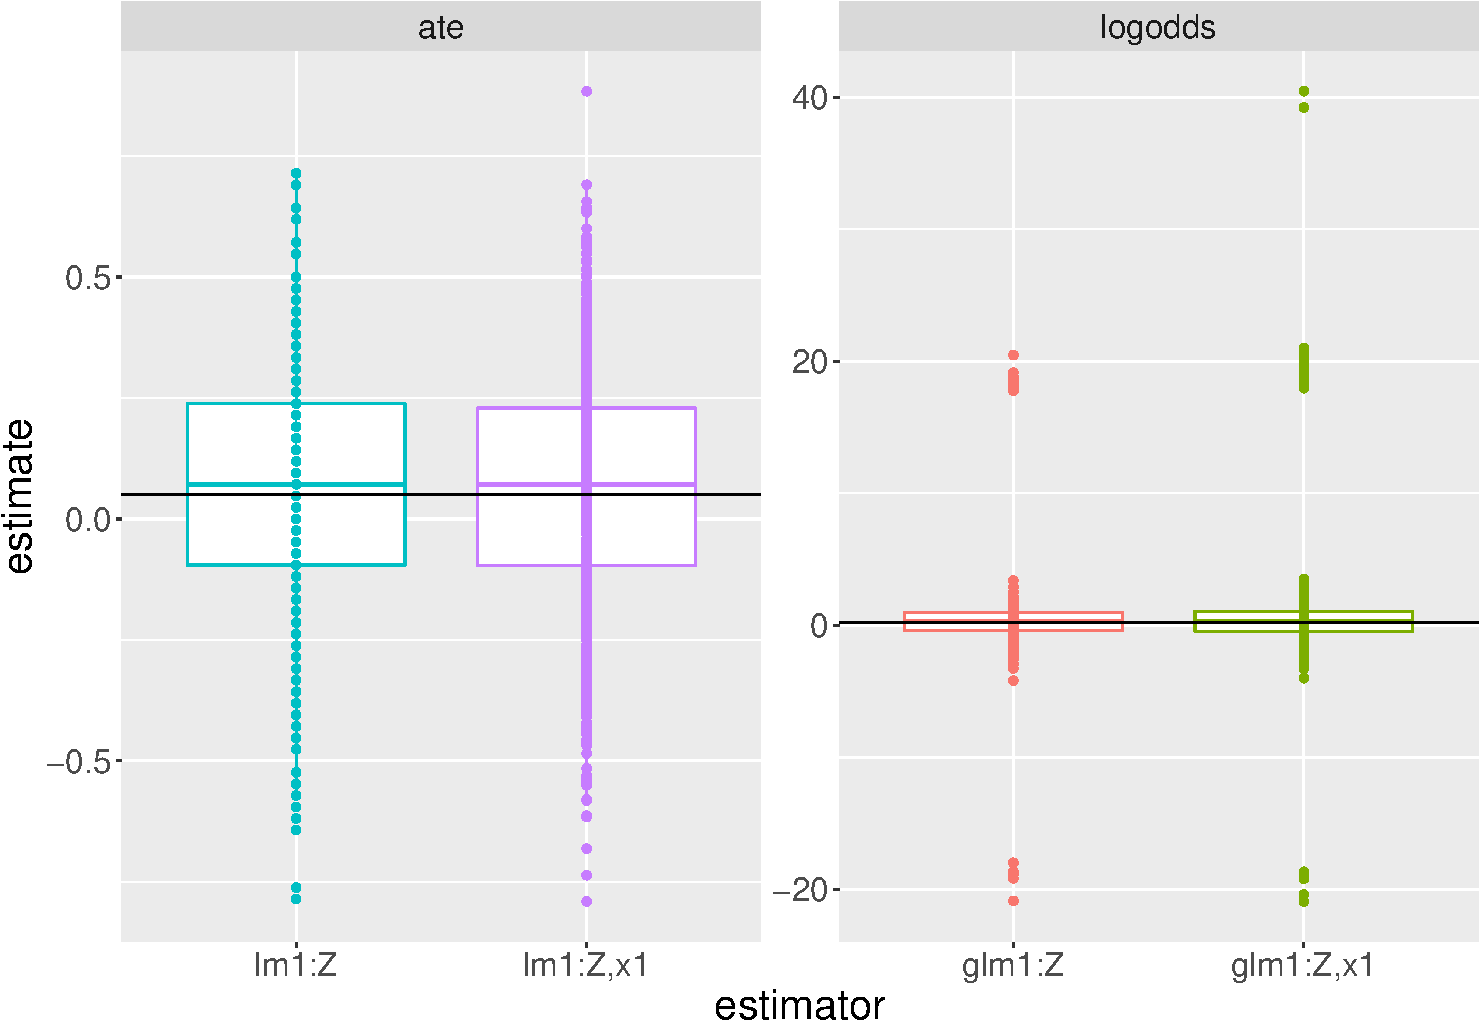
\includegraphics[width=.95\textwidth,]{figs/figsim_plot_bin-1}
\normalsize
\end{frame}

\begin{frame}{Which estimator is closer to the truth?}
\protect\hypertarget{which-estimator-is-closer-to-the-truth-2}{}
Which estimator works better on this design and these data?

\scriptsize\normalsize

\scriptsize

\begin{table}

\caption{\label{tab:showresbin1}Estimator and Test Performance in 5000 simulations of the different estimators and confidence intervals for a binary outcome and completely randomized design.}
\centering
\begin{tabular}[t]{llrrrrrr}
\toprule
est & estimand & bias & rmse & power & coverage & sd\_est & mean\_se\\
\midrule
glm1:Z & logodds & 0.691 & 4.099 & 0.023 & 0.995 & 4.226 & 154.088\\
glm1:Z,x1 & logodds & 0.850 & 4.815 & 0.016 & 0.993 & 4.934 & 249.506\\
lm1:Z & ate & 0.007 & 0.182 & 0.084 & 0.970 & 0.239 & 0.239\\
lm1:Z,x1 & ate & 0.010 & 0.189 & 0.082 & 0.970 & 0.245 & 0.247\\
\bottomrule
\end{tabular}
\end{table}

\normalsize
\end{frame}

\hypertarget{other-topics-in-estimation}{%
\section{Other topics in estimation}\label{other-topics-in-estimation}}

\begin{frame}{Covariance adjustment: Estimands}
\protect\hypertarget{covariance-adjustment-estimands}{}
In general, simply ``controlling for'' produces a biased estimator of
the ATE \textbf{or} ITT estimand. See for example
\protect\hyperlink{ref-lin_agnostic_2013}{Lin}
(\protect\hyperlink{ref-lin_agnostic_2013}{2013}) and
\protect\hyperlink{ref-freedman2008rae}{Freedman}
(\protect\hyperlink{ref-freedman2008rae}{2008a}).
\protect\hyperlink{ref-lin_agnostic_2013}{Lin}
(\protect\hyperlink{ref-lin_agnostic_2013}{2013}) shows how to reduce
this bias and, importantly, that this bias tends to be small as the
sample size increases.
\end{frame}

\hypertarget{conclusion}{%
\section{Conclusion}\label{conclusion}}

\begin{frame}{Final thoughts on basics of estimation}
\protect\hypertarget{final-thoughts-on-basics-of-estimation}{}
\begin{itemize}
\item
  Counterfactual causal estimands are unobserved functions of potential
  outcomes.
\item
  Estimators are recipes or computational formulas that use observed
  data to learn about an estimand.
\item
  Good estimators produce estimates that are close to the true estimand
\item
  (Connecting estimation with testing) Standard errors of estimators
  allow us to calculate confidence intervals and \(p\)-values. Certain
  estimators have larger or smaller (or more or less correct) standard
  errors.
\item
  You can assess the utility of a chosen estimator for a chosen estimand
  by simulation.
\end{itemize}
\end{frame}

\hypertarget{causal-effects-that-differ-by-groups-or-covariates}{%
\section{Causal effects that differ by groups or
covariates}\label{causal-effects-that-differ-by-groups-or-covariates}}

\begin{frame}{Effects that differ by groups I}
\protect\hypertarget{effects-that-differ-by-groups-i}{}
If our theory suggests that effects should differ by group, how can we
assess evidence for or against such claims?

\begin{itemize}
\item
  We can \textbf{design} for an assessment of this theory by creating a
  block-randomized study --- with blocked defined by the theoretically
  relevant groups.
\item
  We can \textbf{plan} for such an assessment by (1)
  \textbf{pre-registering specific subgroup analyses} (whether or not we
  block on that group in the design phase) and (2) making sure to
  measure group membership during baseline data collection pre-treatment
\end{itemize}
\end{frame}

\begin{frame}{Effects that differ by groups II}
\protect\hypertarget{effects-that-differ-by-groups-ii}{}
\begin{itemize}
\item
  If we have not planned ahead, subgroup-specific analyses can be useful
  as explorations but should not be understood as confirmatory: they can
  too easily create problems of testing too many hypotheses thus
  inflated false positive rates.
\item
  We \textbf{should not use groups formed by treatment}. (This is either
  ``mediation analysis'' or ``conditioning on post-treatment variables''
  and deserves its own module).
\end{itemize}
\end{frame}

\hypertarget{causal-effects-when-we-do-not-control-the-dose}{%
\section{Causal effects when we do not control the
dose}\label{causal-effects-when-we-do-not-control-the-dose}}

\begin{frame}{Defining causal effects I}
\protect\hypertarget{defining-causal-effects-i}{}
Imagine a door-to-door communication experiment where some houses are
randomly assigned to receive a visit. Note that we now use \(Z\) and
\(d\) instead of \(T\).

\begin{itemize}
\tightlist
\item
  \(Z_i\) is random assignment to a visit (\(Z_i=1\)) or not
  (\(Z_i=0\)).
\item
  \(d_{i,Z_i=1}=1\) means that person \(i\) would open the door to have
  a conversation when assigned a visit.
\item
  \(d_{i,Z_i=1}=0\) means that person \(i\) would not open the door to
  have a conversation when assigned a visit.
\item
  Opening the door is an outcome of the treatment.
\end{itemize}

\begin{center}
\begin{tikzcd}[ampersand replacement=\&]
Z  \arrow[from=1-1,to=1-2, "\ne 0"] \arrow[from=1-1, to=1-4, bend left, "\text{0 (exclusion)}"] \& d  \arrow[from=1-2,to=1-4] \& \& y \\
(x_1 \ldots x_p) \arrow[from=2-1,to=1-1, "\text{0 (as if randomized)}"]  \arrow[from=2-1,to=1-2] \arrow[from=2-1,to=1-4]
\end{tikzcd}
\end{center}
\end{frame}

\begin{frame}{Defining causal effects II}
\protect\hypertarget{defining-causal-effects-ii}{}
\begin{itemize}
\item
  \(y_{i,Z_i = 1, d_{i,Z_i=1}=1}\) is the potential outcome for people
  who were assigned a visit and who opened the door. (``Compliers'' or
  ``Always-takers'')
\item
  \(y_{i,1, d_{i,Z_i=1}=0}\) is the potential outcome for people who
  were assigned a visit and who did not open the door. (``Never-takers''
  or ``Defiers'')
\item
  \(y_{i,0, d_{i,0}=1}\) is the potential outcome for people who were
  not assigned a visit and who opened the door. (``Defiers'' or
  ``Always-takers'')
\item
  \(y_{i,0, d_{i,0}=0}\) is the potential outcome for people who were
  not assigned a visit and who would not have opened the door.
  (``Compliers'' or ``Never-takers'')
\end{itemize}
\end{frame}

\begin{frame}{Defining causal effects III}
\protect\hypertarget{defining-causal-effects-iii}{}
We could also write \(y_{i,Z_i = 0, d_{i,Z_i=1}=1}\) for people who were
not assigned a visit but who would have opened the door had they been
assigned a visit etc.

In this case we can simplify our potential outcomes:

\begin{itemize}
\tightlist
\item
  \(y_{i,0, d_{i,1}=1} = y_{i,0, d_{i,1}=0} = y_{i,0, d_{i,0}=0}\)
  because your outcome is the same regardless of how you don't open the
  door.
\end{itemize}
\end{frame}

\begin{frame}{Defining causal effects IV}
\protect\hypertarget{defining-causal-effects-iv}{}
We can simplify the ways in which people get a dose of the treatment
like so (where \(d\) is lower case reflecting the idea that whether you
open the door when visited or not is a fixed attribute like a potential
outcome).

\begin{itemize}
\tightlist
\item
  \(Y\) : outcome (\(y_{i,Z}\) or \(y_{i,Z_i=1}\) for potential outcome
  to treatment for person \(i\), fixed)
\item
  \(X\) : covariate/baseline variable
\item
  \(Z\) : treatment assignment (\(Z_i=1\) if assigned to a visit,
  \(Z_i=0\) if not assigned to a visit)
\item
  \(D\) : treatment received (\(D_i=1\) if answered phone, \(D_i=0\) if
  person \(i\) dd not answer the door) (using \(D\) here because
  \(D_i = d_{i,1} Z_{i} + d_{i,0} (1-Z_i)\))
\end{itemize}
\end{frame}

\begin{frame}{Defining causal effects V}
\protect\hypertarget{defining-causal-effects-v}{}
We have two causal effects of \(Z\): \(Z \rightarrow Y\) (\(\delta\),
ITT, ITT\(_Y\)), and \(Z \rightarrow D\) (GG call this ITT\(_D\)).

And different types of people can react differently to the attempt to
move the dose with the instrument.

\centering
\begin{tabular}{llcc}
                       &        & \multicolumn{2}{c}{$Z=1$} \\
               &       & $D=0$ & $D=1$ \\
               \midrule
\multirow{2}{*}{$Z=0$} & $D=0$ & Never taker & Complier \\
                       & $D=1$ & Defier     & Always taker \\
               \bottomrule
\end{tabular}
\end{frame}

\begin{frame}{Defining causal effects VI}
\protect\hypertarget{defining-causal-effects-vi}{}
The \(ITT=ITT_Y=\delta= \bar{y}_{Z=1} - \bar{y}_{Z=0}\).

\medskip

But, in this design, \(\bar{y}_{Z=1}=\bar{y}_{1}\) is split into pieces:
the outcome of those who answered the door (Compliers and Always-takers
and Defiers). Write \(p_C\) for the proportion of compliers in the
study.

\begin{equation}
\bar{y}_{1}=(\bar{y}_{1}|C)p_C + (\bar{y}_{1}|A)p_A + (\bar{y}_1|N)p_N + (\bar{y}_1|D)p_D.
\end{equation}

And \(\bar{y}_{0}\) is also split into pieces:

\begin{equation}
\bar{y}_{0}=(\bar{y}_{0}|C)p_C + (\bar{y}_{1}|A)p_A + (\bar{y}_{0}|N)p_N + (\bar{y}_0|D)p_D.
\end{equation}
\end{frame}

\begin{frame}{Defining causal effects VII}
\protect\hypertarget{defining-causal-effects-vii}{}
So, the ITT itself is a combination of the effects of \(Z\) on \(Y\)
within these different groups (imagine substituting in and then
re-arranging so that we have a set of ITTs, one for each type of
subject). But, we can still estimate it because we have unbiased
estimators of \(\bar{y}_1\) and \(\bar{y}_0\) within each type.
\end{frame}

\begin{frame}{Learning about the ITT I}
\protect\hypertarget{learning-about-the-itt-i}{}
First, let's learn about the effect of the policy itself. To write down
the ITT, we do not need to consider all of the types above. We have no
defiers (\(p_D=0\)) and we know the ITT for both Always-takers and
Never-takers is 0.

\begin{equation}
\bar{y}_{1}=(\bar{y}_{1}|C)p_C + (\bar{y}_{1}|A)p_A + (\bar{y}_1|N)p_N
\end{equation}

\begin{equation}
\bar{y}_{0}=(\bar{y}_{0}|C)p_C + (\bar{y}_{0}|A)p_A + (\bar{y}_{0}|N)p_N
\end{equation}
\end{frame}

\begin{frame}{Learning about the ITT II}
\protect\hypertarget{learning-about-the-itt-ii}{}
First, let's learn about the effect of the policy itself. To write down
the ITT, we do not need to consider all of the types above. We have no
defiers (\(p_D=0\)) and we know the ITT for both Always-takers and
Never-takers is 0.

\begin{align}
ITT    = & \bar{y}_{1} - \bar{y}_{0} \\
        = & ( (\bar{y}_{1}|C)p_C + (\bar{y}_{1}|A)p_A + (\bar{y}_1|N)p_N ) - \\
       & ( (\bar{y}_{0}|C)p_C + (\bar{y}_{0}|A)p_A + (\bar{y}_{0}|N)p_N )  \\
       \intertext{collecting each type together --- to have an ITT for each type}
       = & ( (\bar{y}_{1}|C)p_C -  (\bar{y}_{0}|C)p_C )  +   ( (\bar{y}_{1}|A)p_A - (\bar{y}_{1}|A)p_A ) + \\
       & ( (\bar{y}_1|N)p_N  - (\bar{y}_{0}|N)p_N ) \\
       = & \left( (\bar{y}_{1}|C) -  (\bar{y}_{0}|C) \right)p_C   +  \\
       & \left( (\bar{y}_{1}|A)- (\bar{y}_{0}|A) \right)p_A  +  \left( (\bar{y}_1|N) - (\bar{y}_{0}|N) \right)p_N
\end{align}
\end{frame}

\begin{frame}{Learning about the ITT III}
\protect\hypertarget{learning-about-the-itt-iii}{}
\begin{align}
ITT     = &   \bar{y}_{1} - \bar{y}_{0} \\
        = &  ( (\bar{y}_{1}|C)p_C + (\bar{y}_{1}|A)p_A + (\bar{y}_1|N)p_N ) - \\
       & ( (\bar{y}_{0}|C)p_C + (\bar{y}_{0}|A)p_A + (\bar{y}_{0}|N)p_N )  \\
        = &   ( (\bar{y}_{1}|C)p_C -  (\bar{y}_{0}|C)p_C )  +   ( (\bar{y}_{1}|A)p_A - (\bar{y}_{1}|A)p_A ) + \\
       & ( (\bar{y}_1|N)p_N  - (\bar{y}_{0}|N)p_N ) \\
        = &   ( (\bar{y}_{1}|C) -  (\bar{y}_{0}|C))p_C   +   ( (\bar{y}_{1}|A)- (\bar{y}_{0}|A))p_A  + \\
       & ( (\bar{y}_1|N) - (\bar{y}_{0}|N) )p_N
\end{align}
\end{frame}

\begin{frame}{Learning about the ITT IV}
\protect\hypertarget{learning-about-the-itt-iv}{}
And, if the effect of the dose can only occur for those who open the
door, and you can only open the door when assigned to do so then:

\begin{equation}
( (\bar{y}_{1}|A)- (\bar{y}_{0}|A))p_A = 0  \text{ and } ( (\bar{y}_1|N) - (\bar{y}_{0}|N) )p_N = 0
\end{equation}

And

\begin{equation}
ITT =  ( (\bar{y}_{1}|C) -  (\bar{y}_{0}|C))p_C  = ( CACE ) p_C.
\end{equation}
\end{frame}

\begin{frame}{The complier average causal effect I}
\protect\hypertarget{the-complier-average-causal-effect-i}{}
We would also like to learn about the causal effect of answering the
door and having the conversation, the theoretically interesting effect.

But this comparison is confounded by \(x\): a simple
\(\bar{Y}|D=1 - \bar{Y}|D=0\) comparison tells us about differences in
the outcome due to \(x\) in addition to the difference caused by \(D\).
(Numbers below from some simulated data)

\begin{center}
\begin{tikzcd}[ampersand replacement=\&]
Z  \arrow[from=1-1,to=1-2] \arrow[from=1-1, to=1-4, bend left, "\text{0 (exclusion)}"] \& D  \arrow[from=1-2,to=1-4] \& \& y \\
(x_1 \ldots x_p) \arrow[from=2-1,to=1-1, "\text{-.006 (as if randomized)}"]  \arrow[from=2-1,to=1-2, ".06"] \arrow[from=2-1,to=1-4, ".48"]
\end{tikzcd}
\end{center}
\end{frame}

\begin{frame}[fragile]{The complier average causal effect II}
\protect\hypertarget{the-complier-average-causal-effect-ii}{}
\scriptsize

\begin{Shaded}
\begin{Highlighting}[]
\FunctionTok{with}\NormalTok{(dat, }\FunctionTok{cor}\NormalTok{(Y, x)) }\DocumentationTok{\#\# can be any number}
\FunctionTok{with}\NormalTok{(dat, }\FunctionTok{cor}\NormalTok{(d, x)) }\DocumentationTok{\#\# can be any number}
\FunctionTok{with}\NormalTok{(dat, }\FunctionTok{cor}\NormalTok{(Z, x)) }\DocumentationTok{\#\# should be near 0}
\end{Highlighting}
\end{Shaded}

\normalsize

But we just saw that, in this design, and with these assumptions
(including a SUTVA assumption) that
\(ITT = ( (\bar{y}_{1}|C) - (\bar{y}_{0}|C))p_C = (CACE) p_C\), so we
can define \(CACE=ITT/p_C\).
\end{frame}

\begin{frame}{How to calculate the ITT and CACE/LATE I}
\protect\hypertarget{how-to-calculate-the-itt-and-cacelate-i}{}
\scriptsize\normalsize

Some example data (where we know all potential outcomes):

\scriptsize
\begin{tabular}{r|r|l|r|r|r|r|r|r|r|r|r|r}
\hline
X & u & type & Z & pZ & DZ0 & DZ1 & YD0Z0 & YD1Z0 & YD0Z1 & YD1Z1 & D & Y\\
\hline
4 & 1.95 & Complier & 0 & 0.5 & 0 & 1 & 1.95 & 2.52 & 1.95 & 2.52 & 0 & 1.95\\
\hline
2 & 0.05 & Complier & 1 & 0.5 & 0 & 1 & 0.05 & 0.63 & 0.05 & 0.63 & 1 & 0.63\\
\hline
\end{tabular}

\normalsize
\end{frame}

\begin{frame}[fragile]{How to calculate the ITT and CACE/LATE II}
\protect\hypertarget{how-to-calculate-the-itt-and-cacelate-ii}{}
The ITT and CACE (the parts)

\scriptsize

\begin{Shaded}
\begin{Highlighting}[]
\NormalTok{itt\_y }\OtherTok{\textless{}{-}} \FunctionTok{difference\_in\_means}\NormalTok{(Y }\SpecialCharTok{\textasciitilde{}}\NormalTok{ Z, }\AttributeTok{data =}\NormalTok{ dat0)}
\NormalTok{itt\_y}
\end{Highlighting}
\end{Shaded}

\begin{verbatim}
Design:  Standard 
  Estimate Std. Error t value Pr(>|t|) CI Lower CI Upper    DF
Z  0.08725      0.233  0.3745   0.7089  -0.3752   0.5497 97.97
\end{verbatim}

\begin{Shaded}
\begin{Highlighting}[]
\NormalTok{itt\_d }\OtherTok{\textless{}{-}} \FunctionTok{difference\_in\_means}\NormalTok{(D }\SpecialCharTok{\textasciitilde{}}\NormalTok{ Z, }\AttributeTok{data =}\NormalTok{ dat0)}
\NormalTok{itt\_d}
\end{Highlighting}
\end{Shaded}

\begin{verbatim}
Design:  Standard 
  Estimate Std. Error t value  Pr(>|t|) CI Lower CI Upper    DF
Z     0.68    0.07307   9.307 8.454e-15   0.5348   0.8252 89.31
\end{verbatim}

\normalsize
\end{frame}

\begin{frame}[fragile]{How to calculate the ITT and CACE/LATE III}
\protect\hypertarget{how-to-calculate-the-itt-and-cacelate-iii}{}
All together:\footnote<.->{works when \(Z \rightarrow D\) is not weak
  see \protect\hyperlink{ref-imbens2005robust}{Imbens and Rosenbaum}
  (\protect\hyperlink{ref-imbens2005robust}{2005}) for a cautionary tale}

\scriptsize

\begin{Shaded}
\begin{Highlighting}[]
\NormalTok{cace\_est }\OtherTok{\textless{}{-}} \FunctionTok{iv\_robust}\NormalTok{(Y }\SpecialCharTok{\textasciitilde{}}\NormalTok{ D }\SpecialCharTok{|}\NormalTok{ Z, }\AttributeTok{data =}\NormalTok{ dat0)}
\NormalTok{cace\_est}
\end{Highlighting}
\end{Shaded}

\begin{verbatim}
            Estimate Std. Error t value Pr(>|t|) CI Lower CI Upper DF
(Intercept)   0.3347     0.1912  1.7502  0.08321 -0.04479   0.7142 98
D             0.1283     0.3404  0.3769  0.70705 -0.54727   0.8039 98
\end{verbatim}

\begin{Shaded}
\begin{Highlighting}[]
\DocumentationTok{\#\# Notice same as below:}
\FunctionTok{coef}\NormalTok{(itt\_y)[[}\StringTok{"Z"}\NormalTok{]] }\SpecialCharTok{/} \FunctionTok{coef}\NormalTok{(itt\_d)[[}\StringTok{"Z"}\NormalTok{]]}
\end{Highlighting}
\end{Shaded}

\begin{verbatim}
[1] 0.1283
\end{verbatim}

\normalsize
\end{frame}

\begin{frame}{Summary of Encouragement/Complier/Dose oriented designs:}
\protect\hypertarget{summary-of-encouragementcomplierdose-oriented-designs}{}
\begin{itemize}
\tightlist
\item
  Analyze as you randomized, even when you don't control the dose
\item
  The danger of per-protocol analysis.
\end{itemize}
\end{frame}

\begin{frame}{References}
\protect\hypertarget{references}{}
\hypertarget{refs}{}
\begin{CSLReferences}{1}{0}
\leavevmode\hypertarget{ref-freedman2008rae}{}%
Freedman, David A. 2008a. {``{On regression adjustments to experimental
data}.''} \emph{Advances in Applied Mathematics} 40 (2): 180--93.

\leavevmode\hypertarget{ref-freedman2008randomization}{}%
---------. 2008b. {``Randomization Does Not Justify Logistic
Regression.''} \emph{Statistical Science} 23 (2): 237--49.

\leavevmode\hypertarget{ref-imbens2005robust}{}%
Imbens, G. W., and P. R. Rosenbaum. 2005. {``Robust, Accurate Confidence
Intervals with a Weak Instrument: Quarter of Birth and Education.''}
\emph{Journal of the Royal Statistical Society Series A} 168 (1):
109--26.

\leavevmode\hypertarget{ref-lin_agnostic_2013}{}%
Lin, Winston. 2013. {``Agnostic Notes on Regression Adjustments to
Experimental Data: {Reexamining} {Freedman}'s Critique.''} \emph{The
Annals of Applied Statistics} 7 (1): 295--318.

\end{CSLReferences}
\end{frame}

\end{document}
